\chapter{Differenzierbare Funktionen}
In diesem Kapitel kommen wir zum Kern der Analysis und f\"uhren den Begriff der 
\href{http://de.wikipedia.org/wiki/Differentialrechnung}{\emph{Ableitung}} einer Funktion ein. 
Dies ist der wichtigste Begriff in der Analysis.  Die folgende formale Definition der Ableitung geht auf 
\href{http://de.wikipedia.org/wiki/Augustin-Louis_Cauchy}{Augustin-Louis Cauchy} zur\"uck.


\section{Der Begriff der Ableitung}
\begin{Definition}[Ableitung]
Es sei $D \subseteq \mathbb{R}$ ein Intervall.  
Eine Funktion $f: D \rightarrow \mathbb{R}$ ist im Punkt $\widehat{x} \in D$ \emph{differenzierbar},
wenn der Grenzwert
\\[0.3cm]
\hspace*{1.3cm}
$\lim\limits_{h \rightarrow 0} \bruch{f(\widehat{x} + h) - f(\widehat{x})}{h}$
\\[0.3cm]
existiert.  In diesem Fall definieren wir 
\\[0.3cm]
\hspace*{1.3cm}
$\displaystyle\frac{\mathrm{d}\,f}{\mathrm{d}x}(\widehat{x}) = \lim\limits_{h \rightarrow 0}
\bruch{f(\widehat{x} + h) - f(\widehat{x})}{h}$.
\\[0.3cm]
Wir bezeichnen den Wert $\ds\frac{\mathrm{d}\,f}{\mathrm{d}x}(\widehat{x})$ als die \emph{Ableitung} der
Funktion $f$ an der Stelle $\widehat{x}$.  Gelegentlich werden \\[0.2cm]
wir f\"ur die Ableitung auch die Schreibweise 
$f'(\widehat{x})$ verwenden.
\eod
\end{Definition}


\remark
Beachten Sie, dass wir in der obigen Definition den Ausdruck
\\[0.3cm]
\hspace*{1.3cm} $\bruch{f(\widehat{x} + h) - f(\widehat{x})}{h}$ \\[0.3cm]
als Funktion von $h$ auffassen.  Dieser Ausdruck wird auch als \emph{Differential-Quotient}
bezeichnet.  Er gibt die Steigung einer Sekante an, welche die Funktion $x \mapsto f(x)$
in den Punkten $\widehat{x}$ und $\widehat{x} + h$ schneidet.  Definieren wir 
\\[0.3cm]
\hspace*{1.3cm}
$r(h) := f(\widehat{x} + h) - f(\widehat{x}) - h \cdot \df{f}(\widehat{x})$,
\\[0.3cm]
so gilt einerseits 
\\[0.3cm]
\hspace*{1.3cm}
$\lim\limits_{h \rightarrow 0} \bruch{r(h)}{h} = 
 \lim\limits_{h \rightarrow 0} \bruch{f(\widehat{x} + h) -
  f(\widehat{x})}{h} - \df{f}(\widehat{x}) = \df{f}(\widehat{x}) - \df{f}(\widehat{x}) = 0$,
\\[0.3cm]
und andererseits haben wir 
\\[0.3cm]
\hspace*{1.3cm}
$f(\widehat{x} + h) = f(\widehat{x}) + h \cdot \df{f}(\widehat{x}) + r(h)$.
\pagebreak

\noindent
Die Funktion $r(h)$ ist also der Fehler, der entsteht, wenn wir die Funktion $f(x)$ durch ihre
Tangente im Punkt $\bigl\langle\widehat{x}, f(\widehat{x})\bigr\rangle$ approximieren.  \eox


\remark
Falls die Funktion $f$ im Punkt $\widehat{x}$ differenzierbar ist,
dann ist die Funktion dort auch stetig, denn es gilt 
\\[0.3cm]
\hspace*{1.3cm}
$
\begin{array}[t]{lcl}
\lim\limits_{h \rightarrow 0} f(\widehat{x}+h) & = &
 \lim\limits_{h \rightarrow 0} f(\widehat{x}+h) - f(\widehat{x}) + f(\widehat{x}) \\[0.3cm]
& = & \lim\limits_{h \rightarrow 0} \bruch{f(\widehat{x}+h) - f(\widehat{x})}{h} \cdot h + f(\widehat{x}) \\[0.3cm]
& = & \lim\limits_{h \rightarrow 0} \bruch{f(\widehat{x}+h) - f(\widehat{x})}{h} \cdot \lim\limits_{h \rightarrow 0} h + f(\widehat{x}) \\[0.3cm]
& = & f'(\widehat{x}) \cdot 0 + f(\widehat{x}) \\[0.3cm]
& = & f(\widehat{x})
\end{array}
$
\\[0.3cm]
und $\lim\limits_{h \rightarrow 0} f(\widehat{x}+h) = f(\widehat{x})$ hei{\ss}t gerade, dass $f$
im Punkt $\widehat{x}$ stetig ist. \qed
\vspace*{0.3cm}

\examples
\begin{enumerate}
\item Die konstante Funktion $f := (x \mapsto c)$ hat \"uberall die Ableitung
      $0$, denn es gilt \\[0.3cm]
      \hspace*{1.3cm}$\lim\limits_{h \rightarrow 0} \bruch{f(\widehat{x} + h) - f(\widehat{x})}{h} =
\lim\limits_{h \rightarrow 0} \bruch{c - c}{h} = \lim\limits_{h \rightarrow 0} 0 = 0$.
\item Die identische Funktion $\textsl{id} := (x \mapsto x)$ hat \"uberall die Ableitung 1,
      denn es gilt: 
      \\[0.3cm]
      \hspace*{1.3cm}
      $\lim\limits_{h \rightarrow 0} \bruch{\textsl{id}(\widehat{x} + h) - \textsl{id}(\widehat{x})}{h} =
       \lim\limits_{h \rightarrow 0} \bruch{\widehat{x} + h - \widehat{x}}{h} =
       \lim\limits_{h \rightarrow 0} \bruch{h}{h} = \lim\limits_{h \rightarrow 0} 1 = 1$.
\item Die Funktion $\textsl{abs} := ( x \mapsto |x|)$, die den Absolutbetrag berechnet, ist im
      Punkte $\widehat{x} = 0$ nicht differenzierbar.  Wir zeigen, dass der Grenzwert
      \\[0.3cm]
      \hspace*{1.3cm}
            $\lim\limits_{h \rightarrow 0} \bruch{\textsl{abs}(h) - \textsl{abs}(0)}{h}$
      \\[0.3cm]
      nicht existiert.  Dazu betrachten wir zun\"achst die Folge $\folge{\frac{1}{n}}$.
      Nehmen wir an, dass dieser Grenzwert existiert und den Wert $a$ hat.  
      Da \\[0.3cm]
      \hspace*{1.3cm}
      $\lim\limits_{n\rightarrow\infty} \frac{1}{n} = 0$ 
      \\[0.3cm]
      ist, m\"usste nach Definition des Grenzwerts dann gelten: \\[0.3cm]
      \hspace*{1.3cm}
      $a = \ds \lim\limits_{h \rightarrow 0} \bruch{\textsl{abs}(h) - \textsl{abs}(0)}{h} = 
       \lim\limits_{n\rightarrow\infty} \frac{\textsl{abs}(\frac{1}{n})}{\frac{1}{n}} = 
       \lim\limits_{n\rightarrow\infty} \frac{\;\frac{1}{n}\;}{\frac{1}{n}} = 1 $.
      \\[0.3cm]
      Betrachten wir andererseits die Folge $\folge{-\frac{1}{n}}$ und ber\"ucksichtigen,
      dass diese Folge ebenfalls gegen 0 konvergiert, so erhalten wir
      \\[0.3cm]
      \hspace*{1.3cm}
      $a = \ds \lim\limits_{h \rightarrow 0} \bruch{\textsl{abs}(h) - \textsl{abs}(0)}{h} = 
       \lim\limits_{n\rightarrow\infty} \frac{\textsl{abs}(-\frac{1}{n})}{-\frac{1}{n}} = 
       \lim\limits_{n\rightarrow\infty} \frac{\;\frac{1}{n}\;}{-\frac{1}{n}} = -1$.
      \\[0.3cm]
      Da $a$ nicht gleichzeitig die Werte $+1$ und $-1$ annehmen kann, m\"ussen wir folgern,
      dass die Funktion $\textsl{abs}$ an der Stelle $\widehat{x} = 0$ nicht
      differenzierbar ist.  \eox
\end{enumerate}
\pagebreak

\begin{Satz}[Ableitungs-Regeln]
Es seien $f: D \rightarrow \mathbb{R}$  und $g: D \rightarrow \mathbb{R}$ Funktionen, die
im Punkt $\widehat{x}$ differenzierbar sind. Dann gilt:
\begin{enumerate}
\item Die Funktion $f + g := \bigl(x \mapsto f(x) + g(x)\bigr)$ ist im Punkt $\widehat{x}$
      differenzierbar und es gilt:
      \\[0.3cm]
      \hspace*{1.3cm} $(f+ g)'(\widehat{x}) = f'(\widehat{x}) + g'(\widehat{x})$.
\item Die Funktion $f - g := \bigl(x \mapsto f(x) - g(x)\bigr)$ ist im Punkt $\widehat{x}$
      differenzierbar und es gilt:
      \\[0.3cm]
      \hspace*{1.3cm} $(f - g)'(\widehat{x}) = f'(\widehat{x}) - g'(\widehat{x})$.
\item Die Funktion $f \cdot g := \bigl(x \mapsto f(x) \cdot g(x)\bigr)$ ist im Punkt $\widehat{x}$
      differenzierbar und es gilt die Produkt-Regel:
      \\[0.3cm]
      \hspace*{1.3cm} $(f \cdot g)'(\widehat{x}) = f'(\widehat{x})\cdot g(\widehat{x}) + f(\widehat{x})\cdot g'(\widehat{x})$.
\item Ist $g(\widehat{x}) \not= 0$, dann ist
      die Funktion $\bruch{f}{g} := \Bigl(x \mapsto \bruch{f(x)}{g(x)}\Bigr)$ im Punkt $\widehat{x}$
      differenzierbar und es gilt die Quotienten-Regel:
      \\[0.3cm]
      \hspace*{1.3cm} $\left(\bruch{f}{g}\right)'(\widehat{x}) = \bruch{f'(\widehat{x})\cdot g(\widehat{x}) - f(\widehat{x})\cdot g'(\widehat{x})}{g(\widehat{x})^2}$.
\end{enumerate}
\end{Satz}

\noindent
\textbf{Beweis}: Wir zeigen nur die Produkt-Regel.  Es gilt:
\\[0.3cm]
\hspace*{0.3cm}
$
\begin{array}[t]{lcl}
 &   &  (f \cdot g)'(\widehat{x}) \\[0.2cm]
 & = & \lim\limits_{h \rightarrow 0} \bruch{(f\cdot g)(\widehat{x} + h) - (f\cdot g)(\widehat{x})}{h} \\[0.3cm]
 & = &  \lim\limits_{h \rightarrow 0} \bruch{f(\widehat{x} + h)\cdot g(\widehat{x} + h) - f(\widehat{x})\cdot g(\widehat{x})}{h} \\[0.3cm]
 & = &  \lim\limits_{h \rightarrow 0} \bruch{f(\widehat{x} + h)\cdot g(\widehat{x} + h) - f(\widehat{x})\cdot g(\widehat{x} + h)}{h} + 
                                      \bruch{f(\widehat{x})\cdot g(\widehat{x} + h) - f(\widehat{x})\cdot g(\widehat{x})}{h} \\[0.3cm]
 & = &  \lim\limits_{h \rightarrow 0} \bruch{f(\widehat{x} + h)\cdot g(\widehat{x} + h) - f(\widehat{x})\cdot g(\widehat{x} + h)}{h} +
        \lim\limits_{h \rightarrow 0} \bruch{f(\widehat{x})\cdot g(\widehat{x} + h) - f(\widehat{x})\cdot g(\widehat{x})}{h} \\[0.3cm]
 & = &  \lim\limits_{h \rightarrow 0} \bruch{f(\widehat{x} + h) - f(\widehat{x})}{h} \cdot \lim\limits_{h \rightarrow 0} g(\widehat{x}+h) +
        \lim\limits_{h \rightarrow 0} f(\widehat{x}) \cdot \lim\limits_{h \rightarrow 0} \bruch{g(\widehat{x} + h) - g(\widehat{x})}{h} \\[0.4cm]
 & = &  f'(\widehat{x}) \cdot  g(\widehat{x}) + f(\widehat{x}) \cdot g'(\widehat{x}) \\[0.3cm]
\end{array}
$
\\[0.3cm]
Dabei haben wir im letzten Schritt ausgenutzt, dass eine differenzierbare Funktion auch stetig ist.
Daher gilt 
\\[0.2cm]
\hspace*{1.3cm}
$\lim\limits_{h \rightarrow 0} g(\widehat{x} + h) = g(\widehat{x})$. \hspace*{\fill} $\Box$
\vspace*{0.3cm}

\exercise
Zeigen Sie: Ist die Funktion $g$ im Punkt $\widehat{x}$ differenzierbar und gilt
$g(\widehat{x}) \not= 0$, so ist auch die Funktion 
$\bruch{1}{g} := \left(x \mapsto \bruch{1}{g(x)}\right)$ im Punkt $\widehat{x}$
differenzierbar und es gilt 
\\[0.3cm]
\hspace*{1.3cm} 
$\left(\bruch{1}{g}\right)'(\widehat{x}) = -\bruch{g'(\widehat{x})}{g(\widehat{x})^2}$.
\\[0.3cm]
Folgern Sie aus diesem Ergebnis die Quotienten-Regel.
\eox
\pagebreak

\begin{Satz}[Ketten-Regel] 
  Die Funktionen $f:\mathbb{R} \rightarrow \mathbb{R}$ 
  sei differenzierbar im Punkt $\widehat{x}\in\mathbb{R}$ und die Funktion
  $g:\mathbb{R} \rightarrow \mathbb{R}$ sei differenzierbar im Punkt 
  $\widehat{y} = f(\widehat{x})$.  Dann ist auch die Funktion
  \\[0.2cm]
  \hspace*{1.3cm}
  $g \circ f := \bigr(x \mapsto g(f(x))\bigr)$ 
  \\[0.2cm]
  im Punkt $\widehat{x}$  differenzierbar und es gilt 
  \\[0.3cm]
  \hspace*{1.3cm}
  $(g\circ f)'(\widehat{x}) = g'(f(\widehat{x})) \cdot f'(\widehat{x})$.  
\end{Satz}

\noindent
\textbf{Beweis}: 
Aus der Differenzierbarkeit von $f$ und $g$ folgt, dass es Funktionen $r_1(h)$ und
$r_2(h)$ gibt, so dass gilt:
\begin{enumerate}
\item $f(\widehat{x}+h) = f(\widehat{x}) + h\cdot f'(\widehat{x}) + r_1(h)$ \quad mit $\lim\limits_{h \rightarrow 0} \bruch{r_1(h)}{h} = 0$,
\item $g(\widehat{y}+h) = g(\widehat{y}) + h\cdot g'(\widehat{y}) + r_2(h)$ \quad mit $\lim\limits_{h \rightarrow 0} \bruch{r_2(h)}{h} = 0$.
\end{enumerate}
Damit finden wir f\"ur den Differential-Quotienten der Funktion $g \circ f$ im Punkt
$\widehat{x}$: \\[0.3cm]
\hspace*{1.3cm}
$
\begin{array}[t]{lcl}
& & \bruch{(g\circ f)(\widehat{x} + h) - (g\circ f)(\widehat{x})}{h} \\[0.3cm]
&=& \bruch{g\bigl(f(\widehat{x} + h)\bigr) - g\bigl(f(\widehat{x})\bigr)}{h} \\[0.3cm]
&=& \bruch{g\bigl(f(\widehat{x}) + h\cdot f'(\widehat{x}) + r_1(h)\bigr) - g\bigl(f(\widehat{x})\bigr)}{h} \\[0.3cm]
&=& \bruch{g\bigl(\widehat{y} + h\cdot f'(\widehat{x}) + r_1(h)\bigr) - g\bigl(\widehat{y}\bigr)}{h} \\[0.3cm]
&=& \bruch{g(\widehat{y}) + \bigl(h\cdot f'(\widehat{x}) + r_1(h)\bigr)\cdot g'(\widehat{y}) + r_2\bigl(h\cdot f'(\widehat{x}) + r_1(h)\bigr) - g(\widehat{y})}{h} \\[0.3cm]
&=& f'(\widehat{x})\cdot g'(\widehat{y}) + \bruch{r_1(h)}{h}\cdot g'(\widehat{y}) + \bruch{r_2\bigl(h\cdot f'(\widehat{x}) + r_1(h)\bigr)}{h} \\[0.3cm]
\end{array}
$
\\[0.3cm]
Wenn wir jetzt den Grenzwert $h \rightarrow 0$ berechnen, dann m\"ussen wir uns den letzten
Term genauer ansehen. Es gilt 
\\[0.3cm] 
\hspace*{1.3cm}
 $
 \begin{array}[t]{lcl}
 \lim\limits_{h \rightarrow 0}\bruch{r_2\bigl(h\cdot f'(\widehat{x}) + r_1(h)\bigr)}{h} &=&
 \lim\limits_{h \rightarrow 0}\bruch{r_2\bigl(h\cdot f'(\widehat{x}) + r_1(h)\bigr)}{h\cdot f'(\widehat{x}) + r_1(h)} \cdot \bruch{h\cdot f'(\widehat{x}) + r_1(h)}{h} \\[0.5cm]
& = & \lim\limits_{h \rightarrow 0}\bruch{r_2\bigl(h\cdot f'(\widehat{x}) + r_1(h)\bigr)}{h\cdot f'(\widehat{x}) + r_1(h)} \cdot 
      \lim\limits_{h \rightarrow 0} \bruch{h\cdot f'(\widehat{x}) + r_1(h)}{h} \\[0.5cm]
& = & \lim\limits_{h \rightarrow 0}\bruch{r_2\bigl(h\bigr)}{h} \cdot 
      \left(\lim\limits_{h \rightarrow 0} f'(\widehat{x}) + \bruch{r_1(h)}{h}\right) \\[0.5cm]
& = & 0 \cdot \bigl(f'(\widehat{x}) + 0\bigr) \\[0.2cm]
& = & 0
\end{array}
$
\\[0.3cm]
Damit sehen wir:
\\[0.3cm]
\hspace*{1.3cm}
$
\begin{array}[t]{lcl}
 & & \lim\limits_{h \rightarrow 0} \bruch{(g\circ f)(\widehat{x} + h) - (g\circ f)(\widehat{x})}{h} \\[0.5cm]
 & = & \lim\limits_{h \rightarrow 0} f'(\widehat{x})\cdot g'(\widehat{y}) + \bruch{r_1(h)}{h}\cdot g'(\widehat{y}) + \bruch{r_2\bigl(h\cdot f'(\widehat{x}) + r_1(h)\bigr)}{h} \\[0.5cm]
 &=& f'(\widehat{x})\cdot g'(\widehat{y}) + \lim\limits_{h \rightarrow 0} \bruch{r_1(h)}{h}\cdot g'(\widehat{y}) + \lim\limits_{h \rightarrow 0} \bruch{r_2\bigl(h\cdot f'(\widehat{x}) + r_1(h)\bigr)}{h} \\[0.5cm]
 &=& f'(\widehat{x})\cdot g'(\widehat{y}) + 0 + 0 \\[0.3cm]
 &=& f'(\widehat{x})\cdot g'(\widehat{y}).
\end{array}
$
\\[0.3cm]
Der obige exakte Beweis ist recht umst\"andlich.  Wir geben daher zus\"atzlich eine
Plausibilit\"atsbetrachtung.  Nach Definition der Ableitung gilt 
\\[0.3cm]
\hspace*{1.3cm}
$g'(\widehat{y}) = \lim\limits_{h \rightarrow 0} \bruch{g(\widehat{y} + h) - g(\widehat{y})}{h}$
\\[0.3cm]
F\"ur kleine Werte von $h$ gilt daher ungef\"ahr 
\\[0.2cm]
\hspace*{1.3cm}
$g(\widehat{y} + h) \approx g(\widehat{y}) + g'(\widehat{y})\cdot h$.
\\[0.2cm]
Analog finden wir f\"ur die Funktion $f$
\\[0.2cm]
\hspace*{1.3cm}
$f(\widehat{x} + h) \approx f(\widehat{x}) + f'(\widehat{x})\cdot h$.
\\[0.2cm]
Damit finden wir f\"ur den Differential-Quotienten der Funktion $g \circ f$ im Punkt
$\widehat{x}$: \\[0.3cm]
\hspace*{1.3cm}
$
\begin{array}[t]{lcl}
 \bruch{(g\circ f)(\widehat{x} + h) - (g\circ f)(\widehat{x})}{h} 
&=& \bruch{g\bigl(f(\widehat{x} + h)\bigr) - g\bigl(f(\widehat{x})\bigr)}{h} \\[0.3cm]
&\approx& \bruch{g\bigl(f(\widehat{x}) + f'(\widehat{x})\cdot h\bigr) - g\bigl(f(\widehat{x})\bigr)}{h} \\[0.3cm]
&\approx& \bruch{g\bigl(f(\widehat{x})\bigr) + g'\bigl(f(\widehat{x})\bigr)\cdot f'(\widehat{x})\cdot h - g\bigl(f(\widehat{x})\bigr)}{h} \\[0.3cm]
&=& \bruch{g'\bigl(f(\widehat{x})\bigr)\cdot f'(\widehat{x})\cdot h}{h} \\[0.3cm]
&=& g'\bigl(f(\widehat{x})\bigr)\cdot f'(\widehat{x}) \\[0.3cm]
\end{array}
$
\\[0.3cm]
Die linke Seite der Gleichung stellt den Differential-Quotienten der Funktion $g\circ f$
dar und muss daher f\"ur $h \rightarrow 0$ gegen die Ableitung $(g \circ f)(\widehat{x})$
konvergieren. \hspace*{\fill} $\Box$


\exercise
 Zeigen Sie, dass f\"ur alle nat\"urlichen Zahlen $n$ gilt: 
\\[0.3cm]
\hspace*{1.3cm}
$\ds\frac{d\,x^n}{dx} = n \cdot x^{n-1}$.
\eox

\begin{Satz}[Ableitung von Potenzreihen]
Ist die Funktion $f$ als Potenzreihe definiert, 
\\[0.3cm]
\hspace*{1.3cm} $\sum\limits_{n=0}^\infty a_n \cdot  x^n$ 
\\[0.3cm]
und ist $R$ der Konvergenz-Radius dieser Potenzreihe, so ist $f$ f\"ur alle $x\in\mathbb{R}$
mit $|x| < R$ differenzierbar und es gilt 
\\[0.3cm]
\hspace*{1.3cm} $f'(x) = \sum\limits_{n=1}^\infty n \cdot a_n \cdot x^{n-1}$.
\end{Satz}
\pagebreak

\remark
Der letzte Satz besagt, dass Potenzreihen innerhalb ihres Konvergenz-Radius gliedweise
differenziert werden k\"onnen.   Ein Beweis dieses Satzes ist mit den uns zur Verf\"ugung
stehenden Hilfsmitteln nicht m\"oglich, da uns der Begriff der
\href{https://de.wikipedia.org/wiki/Gleichm��ige_Konvergenz}{\emph{gleichm\"a{\ss}igen Konvergenz}}
einer Funktionen-Folge fehlt und wir nicht die Zeit haben, diesen Begrif einzuf\"uhren.  Um  Ihnen
zu zeigen, dass es an dieser Stelle durchaus Probleme geben k\"onnte, pr\"asentiere ich ein
Beispiel, welches zeigt, dass  
Grenzwertprozesse im Allgemeinen nicht ohne weitere Voraussetzungen vertauscht werden d\"urfen.
Dazu definieren wir f\"ur alle $n \in \mathbb{N}$ die Funktion $f_n:\mathbb{R} \rightarrow \mathbb{R}$ als
\\[0.2cm]
\hspace*{1.3cm}
$\ds f_n(x) := \frac{\;\sin(n \cdot x)\;}{n}$.
\\[0.2cm]
Aus der Tatsache, dass $|\sin(x)| \leq 1$ ist f\"ur alle $x\in \mathbb{R}$ folgt
\\[0.2cm]
\hspace*{1.3cm}
$g(x) := \ds\lim\limits_{n\rightarrow\infty} f_n(x) = \lim\limits_{n\rightarrow\infty} \frac{\;\sin(n \cdot x)\;}{n} = 0$. 
\\[0.2cm]
Wir definieren f\"ur alle $n\in\mathbb{N}$ die Funktion $g_n(x)$ als die Ableitung der Funktion $f_n(x)$:
\\[0.2cm]
\hspace*{1.3cm}
$g_n(x) := f_n'(x) = \cos(n \cdot x)$.
\\[0.2cm]
Wenn wir den Limes $n \rightarrow \infty$ mit dem Differenzieren vertauschen d\"urften, dann
w\"urden wir erwarten, dass 
\\[0.2cm]
\hspace*{1.3cm}
$
\begin{array}[t]{lcl}
g(x) & = & \ds \df{} \lim\limits_{n\rightarrow\infty} \frac{\;\sin(n \cdot x)\;}{n} \\[0.4cm]
     & = & \lim\limits_{n\rightarrow\infty} \df{} \frac{\;\sin(n \cdot x)\;}{n} \\[0.4cm]
     & = & \ds \lim\limits_{n\rightarrow\infty} \cos(n \cdot x) 
\end{array}
$
\\[0.2cm]
gelten w\"urde.  
F\"ur $x = 0$ gilt aber
\\[0.2cm]
\hspace*{1.3cm}
$\lim\limits_{n\rightarrow\infty} \;\cos(n \cdot 0) = \cos(0) = 1 \not= 0 = g(0)$.
\\[0.2cm]
Dieses Beispiel zeigt, dass Grenzwertprozesse im Allgemeinen \underline{nicht} vertauscht werden
d\"urfen. 
\eox

\examples
Wir berechnen als n\"achstes die Ableitung einiger wichtiger Funktionen.  
\begin{enumerate}
\item Die Exponential-Funktion $\exp(x)$ ist definiert als 
      \\[0.3cm]
      \hspace*{1.3cm}
      $\ds\exp(x) = \sum\limits_{n=0}^\infty \bruch{x^n}{n!}$.
      \\[0.3cm]
      Nach dem letzten Satz gilt f\"ur die Ableitung der Exponential-Funktion 
      \\[0.3cm]
      \hspace*{1.3cm}
      $\ds
         \df{}\exp(x) = \sum\limits_{n=1}^\infty \bruch{n}{n!} \cdot x^{n-1}
                             = \sum\limits_{n=1}^\infty \bruch{1}{(n-1)!} \cdot x^{n-1}
                             = \sum\limits_{n=0}^\infty \bruch{1}{n!} \cdot x^{n} = \exp(x)$,
      \\[0.3cm]
      die Ableitung der Exponential-Funktion ergibt also wieder die Exponential-Funktion!
\item Um den nat\"urlichen Logarithmus ableiten zu k\"onnen, betrachten wir die Gleichung 
      \\[0.3cm]
      \hspace*{1.3cm}
      $\ln\bigl(\exp(x)\bigr) = x$.
      \\[0.3cm]
      Differenzieren wir beide Seiten dieser Gleichung nach $x$, so erhalten wir nach der Ketten-Regel
      \\[0.3cm]
      \hspace*{1.3cm}
      $\ds\ln'\bigl(\exp(x)\bigr)\cdot \exp(x) = 1$,
      \\[0.3cm]
      denn die Ableitung der Exponential-Funktion ergibt ja wieder die
      Exponential-Funktion.  Setzen wir hier $y:= \exp(x)$, so haben wir 
      \\[0.3cm]
      \hspace*{1.3cm}
      $\ds\ln'(y) \cdot y = 1$, \quad also \quad
      $\ds\frac{\mathrm{d}\;}{\mathrm{d}y}\ln(y) = \frac{1}{y}$.

      \remark
      An dieser Stelle haben wir nicht gezeigt, dass der nat\"urliche Logarithmus differenzierbar
      ist.  Wir haben lediglich gezeigt, dass unter der Annahme, dass der nat\"urliche Logarithmus
      differenzierbar ist, die Gleichung 
      \\[0.2cm]
      \hspace*{1.3cm}
      $\ds \df{}\ln(x) = \frac{1}{x}$
      \\[0.2cm]
      gefolgert werden kann.  \eox
      

 

      \begin{figure}[!h]
        \centering
        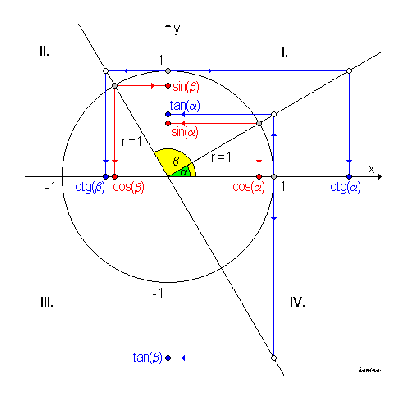
\epsfig{file=Figures/circle.eps,scale=1.5}
        \caption{Die Winkel-Funktionen am Einheitskreis.}
        \label{fig:circle}
      \end{figure}
\item Um die Ableitung der Funktion $x \mapsto \sin(x)$ berechnen zu k\"onnen, 
      betrachten wir in Abbildung \ref{fig:circle} auf Seite \pageref{fig:circle} die Definition von
      Sinus und Tangens am Einheitskreis.  Aus der Definition von Sinus und Tangens folgt die Ungleichung 
      \\[0.3cm]
      \hspace*{1.3cm}
      $\sin(\varphi) \leq \varphi \leq \tan(\varphi) = \bruch{\sin(\varphi)}{\cos(\varphi)}$
      \\[0.3cm]
      Division dieser Gleichung durch $\sin(\varphi)$ liefert
      \\[0.3cm]
      \hspace*{1.3cm}
      $1 \leq \bruch{\varphi}{\sin(\varphi)} \leq \bruch{1}{\cos(\varphi)}$
      \\[0.3cm]
      Wir bilden den Kehrwert und erhalten
      \\[0.3cm]
      \hspace*{1.3cm}
      $1 \geq \bruch{\sin(\varphi)}{\varphi} \geq \cos(\varphi)$
      \\[0.3cm]
      Nun bilden wir den Grenzwert f\"ur $\varphi \rightarrow 0$:
      \\[0.3cm]
      \hspace*{1.3cm}
      $1 \geq \lim\limits_{\varphi \rightarrow 0} \bruch{\sin(\varphi)}{\varphi} \geq \lim\limits_{\varphi \rightarrow 0}\cos(\varphi)$
      \\[0.3cm]
      Wegen $\lim\limits_{\varphi \rightarrow 0} \cos(\varphi) = \cos(0) = 1$ folgt daraus
      \\[0.1cm]
      \hspace*{1.3cm}
      $\lim\limits_{\varphi \rightarrow 0} \bruch{\sin(\varphi)}{\varphi} = 1$.
      \\[0.3cm]
       Aus dem Geometrie-Untericht ist das Additionstheorem f\"ur den Sinus 
       bekannt: 
       \\[0.3cm]
       \hspace*{1.3cm} $\sin(x+y) = \sin(x) \cdot \cos(y) + \cos(x) \cdot \sin(y)$.
         \\[0.2cm]
       Daraus folgt einerseits
       \\[0.3cm]
       \hspace*{1.3cm}
       $
       \begin{array}[t]{lcl}
         \sin(x) & = & \sin\left(\frac{x + y}{2} + \frac{x - y}{2}\right) \\[0.3cm]
                 & = & \sin\left(\frac{x + y}{2}\right)\cdot \cos\left(\frac{x - y}{2}\right) + \cos\left(\frac{x + y}{2}\right)\cdot \sin\left(\frac{x - y}{2}\right) 
       \end{array}
       $
       \\[0.3cm]
       und andererseits gilt wegen $\sin(-x) = -\sin(x)$ und $\cos(-x) = \cos(x)$
       \\[0.3cm]
       \hspace*{1.3cm}
       $
       \begin{array}[t]{lcl}
         \sin(y) & = & \sin\left(\frac{x + y}{2} - \frac{x - y}{2}\right) \\[0.3cm]
                 & = & \sin\left(\frac{x + y}{2}\right)\cdot \cos\left(\frac{x - y}{2}\right) - \cos\left(\frac{x + y}{2}\right)\cdot \sin\left(\frac{x - y}{2}\right). 
       \end{array}
       $
       \\[0.3cm]
       Subtrahieren wir diese Gleichungen voneinander, so erhalten wir 
       \\[0.3cm]
       \hspace*{1.3cm}
       $\sin(x) - \sin(y) = 2 \cdot \cos\left(\frac{x + y}{2}\right)\cdot \sin\left(\frac{x - y}{2}\right)$.
       \\[0.3cm]
       Damit k\"onnen wir die Ableitung des Sinus ausrechnen:
       \\[0.3cm]
       \hspace*{1.3cm}
       $
       \begin{array}[t]{lcl}
       \lim\limits_{h \rightarrow 0} \bruch{\sin(x+h)-\sin(x)}{h} & = &
       \lim\limits_{h \rightarrow 0} \bruch{2 \cdot \cos\left(\frac{x + h + x}{2}\right)\cdot \sin\left(\frac{x + h - x}{2}\right)}{h} \\[0.3cm]
        & = &
        \ds\lim\limits_{h \rightarrow 0} \cos\left(x + \frac{h}{2}\right) \cdot \lim\limits_{h \rightarrow 0} \bruch{\sin\left(\frac{h}{2}\right)}{\frac{h}{2}} \\[0.3cm]
        & = & \cos(x) \cdot \lim\limits_{h \rightarrow 0} \bruch{\sin\left(h\right)}{h} \\[0.3cm]
        & = & \cos(x) \\[0.3cm]
       \end{array}
       $
      \\[0.3cm]
      Damit haben wir gezeigt, dass gilt:
      \\[0.3cm]
      \hspace*{1.3cm}
      $\ds\df{}\sin(x) = \cos(x)$.
\item Die Ableitung des Kosinus k\"onnte in analoger Weise berechnet werden, es ist aber 
      einfacher, wenn wir von den Gleichungen
      \\[0.3cm]
      \hspace*{1.3cm}
      $\cos(x) = \sin\bigl(\frac{\pi}{2}- x\bigr)$ \quad und \quad $\cos(\frac{\pi}{2}- x\bigr) = \sin(x)$
      \\[0.3cm]
      ausgehen und die Ketten-Regel verwenden. Es ergibt sich
      \\[0.3cm]
      \hspace*{1.3cm}
      $
      \begin{array}[t]{lcll}
      \dfo\cos(x) & = & \dfo\sin\Bigl(\frac{\pi}{2}- x\Bigr) \\[0.3cm]
                 & = & \ds\cos\Bigl(\frac{\pi}{2}- x\Bigr) \cdot \dfo\Bigl(\frac{\pi}{2}- x\Bigr) & \mbox{nach der Ketten-Regel} \\[0.3cm]
                 & = & \sin(x) \cdot (-1) \\[0.3cm]
                 & = & -\,\sin(x). \\[0.3cm]
      \end{array}$
\item Jetzt kann die Ableitung der Tangens-Funktion \"uber die Quotienten-Regel berechnet 
      werden: 
      \\[0.3cm]
      \hspace*{1.3cm}
      $\ds
      \begin{array}[t]{lcl}
      \ds \df{} \tan(x) & = & \ds\df{} \left(\bruch{\sin(x)}{\cos(x)}\right) \\[0.3cm]
      & = & \bruch{\Bigl(\df{} \sin(x)\Bigr) \cdot \cos(x) - \sin(x) \cdot \Bigl(\df{} \cos(x)\Bigr)}{\cos^2(x)} \\[0.5cm]
      & = & \bruch{\cos(x) \cdot \cos(x) - \sin(x) \cdot \bigr(-\sin(x)\bigr)}{\cos^2(x)} \\[0.5cm]
      & = & \bruch{\cos^2(x) + \sin^2(x)}{\cos^2(x)} \\[0.5cm]
      & = & \bruch{1}{\cos^2(x)} = \sec^2(x) 
      \end{array}
      $
\item Die Ableitung der Arcus-Tangens-Funktion kann nun mit dem selben Trick berechnet werden,
      den wir schon bei der Berechnung der Ableitung des Logarithmus benutzt haben.
      Wir gehen diesmal von der Gleichungen 
      \\[0.2cm]
      \hspace*{1.3cm}
      $\arctan\bigl(\tan(x)\bigr) = x$
      \\[0.2cm]
      aus und differenzieren beide Seiten dieser Gleichung.  Nach der Ketten-Regel erhalten wir 
      \\[0.3cm]
      \hspace*{1.3cm}
      $\arctan'\bigl(\tan(x)\bigr) \cdot \df{} \tan(x) = 1$.
      \\[0.3cm]
      Setzen wir hier die Ableitung f\"ur die Tangens-Funktion ein, so haben wir
      \\[0.3cm]
      \hspace*{1.3cm}
      $\ds \df{} \arctan\bigl(\tan(x)\bigr) \cdot \bruch{1}{\cos^2(x)} = 1$.
      \\[0.3cm]
      Multiplikation mit $\cos^2(x)$ ergibt
      \\[0.3cm]
      \hspace*{1.3cm}
      $\ds \df{} \arctan\bigl(\tan(x)\bigr) = \cos^2(x)$.
      \\[0.3cm]
      Den in dieser  Gleichung auftretenden Term $\cos^2(x)$ m\"ussen wir durch einen Term ausdr\"ucken, in dem
      nur $\tan(x)$ auftritt.  Dazu betrachten wir die Definition der Tangens-Funktion:      
      \\[0.3cm]
      \hspace*{1.3cm}
      $
      \begin{array}[t]{lrcll}
                & \tan^2(x) & = & \bruch{\sin^2(x)}{\cos^2(x)} \\[0.5cm] 
\Leftrightarrow & \tan^2(x) & = & \bruch{1 - \cos^2(x)}{\cos^2(x)} & \mbox{wegen}\; \sin^2(x) + \cos^2(x) = 1 \\[0.5cm] 
\Leftrightarrow & \cos^2(x) \cdot \tan^2(x) & = & 1 - \cos^2(x) &  \\[0.3cm] 
\Leftrightarrow & \cos^2(x) \cdot \tan^2(x) + \cos^2(x) & = & 1  &  \\[0.3cm] 
\Leftrightarrow & \cos^2(x) \cdot \bigr(\tan^2(x) + 1\bigr) & = & 1  &  \\[0.3cm] 
\Leftrightarrow & \cos^2(x)  & = &  \bruch{1}{\tan^2(x) + 1} &  
      \end{array}
      $
      \\[0.3cm]
      Damit k\"onnen wir also schreiben 
      \\[0.3cm]
      \hspace*{1.3cm}
      $\arctan'\bigl(\tan(x)\bigr) = \bruch{1}{\tan^2(x) + 1}$.
      \\[0.3cm]
      Setzen wir jetzt $y = \tan(x)$, so erhalten wir 
      \\[0.3cm]
      \hspace*{1.3cm}
      $\ds\frac{\mathrm{d}\;}{\mathrm{d}y} \arctan(y) = \bruch{1}{y^2 + 1}$.
\end{enumerate}

\exercise
\begin{enumerate}[(a)]
\item Zeigen Sie 
      \\[0.3cm]
      \hspace*{1.3cm} 
      $\ds\df{} \arcsin(x) = \bruch{1}{\sqrt{1 - x^2}}$.  
\item Zeigen Sie 
      \\[0.3cm]
      \hspace*{1.3cm} 
      $\ds\df{} \arccos(x) = -\bruch{1}{\sqrt{1 - x^2}}$.   \eox
\end{enumerate}


\exercise
Der Sekans eines Winkels $\varphi$ ist als
\\[0.2cm]
\hspace*{1.3cm}
$\ds \sec(\varphi) := \frac{1}{\cos(\varphi)}$
\\[0.2cm]
definiert.  Entsprechend ist der Kosekans eines Winkels $\varphi$ als
\\[0.2cm]
\hspace*{1.3cm}
$\ds \csc(\varphi) := \frac{1}{\sin(\varphi)}$
\\[0.2cm]
definiert.  Beweisen Sie die Gleichungen
\\[0.2cm]
\hspace*{1.3cm}
$\ds \df{} \sec(x) = \sec(x) \cdot \tan(x)$ \quad und \quad
$\ds \df{} \csc(x) = -\csc(x) \cdot \cot(x)$. 
\eox
\vspace*{0.2cm}

\exercise
\begin{enumerate}[(a)]
\item Berechnen Sie die Ableitung der Funktion $x \mapsto \sqrt{x}$.  

      \textbf{Hinweis}: Verwenden Sie die Produkt-Regel. 
\item Es sei $p \in \mathbb{Z}$ und $q \in \mathbb{N}$.  \"Uberlegen Sie, was die Ableitung der Funktion
      \\[0.2cm]
      \hspace*{1.3cm}
      $\ds x \mapsto x^{\normalsize\frac{p}{q}}$
      \\[0.2cm]
      ist und beweisen Sie Ihre Behauptung.

      \textbf{Hinweis}: Betrachten Sie zun\"achst den Fall $p = 1$.  \eox
\end{enumerate}

\section{Mittelwert-S\"atze}
\begin{Definition}[lokales Maximum] \lb
  Eine Funktion $f:\mathbb{R} \rightarrow \mathbb{R}$ hat im Punkt $\bar{x}\in \mathbb{R}$ genau dann ein \emph{lokales Maximum}, wenn 
  \\[0.2cm]
  \hspace*{1.3cm}
  $\exists \varepsilon \in \mathbb{R}_+:\forall x \in \mathbb{R}: 
    \bigl(|x - \bar{x}| < \varepsilon \rightarrow f(x) \leq f(\bar{x})\bigr)
   $
  \\[0.2cm]
  gilt.
  \eod
\end{Definition}

Die in der obigen Definition auftretende Menge von Zahlen, deren Abstand von $\bar{x}$
kleiner ist als $\varepsilon$, bezeichnen wir auch als $\varepsilon$-Umgebung des Punktes
$\bar{x}$, die $\varepsilon$-Umgebung des Punktes $x$ ist also die Menge 
\\[0.2cm]
\hspace*{1.3cm} $U_\varepsilon(\bar{x}) := \bigl\{ x \in \mathbb{R} \;\big|\; |x - \bar{x}| < \varepsilon \bigr\}$.
\\[0.2cm]
Der Begriff des lokalen Maximums steht im Kontrast zu dem Begriff eines \emph{globalen Maximums}.
Eine Funktion $f:D \rightarrow \mathbb{R}$ hat in einem Punkt $\bar{x} \in D$ ein globales
Maximum, wenn
\\[0.2cm]
\hspace*{1.3cm}
$\forall x \in D: f(x) \leq f(\bar{x})$
\\[0.2cm]
gilt.  Nat\"urlich ist jedes globale Maximum auch ein lokales Maximum, aber die Umkehrung
gilt im allgemeinen nicht.  Der n\"achste Satz liefert ein notwendiges Kriterium f\"ur das
Auftreten eines lokalen Maximums.

\begin{Satz}[\href{http://en.wikipedia.org/wiki/Fermat}{Pierre de Fermat}, 160?--1665] \lb
Hat die Funktion $f: D \rightarrow \mathbb{R}$ im Punkt $\bar{x}$ ein lokales
Maximum, ist $U_\varepsilon(\bar{x}) \subseteq D$ und ist die Funktion $f$ zus\"atzlich im Punkt $\bar{x}$ differenzierbar, so gilt 
\\[0.3cm]
\hspace*{1.3cm}
$\df{f}(\bar{x}) = 0$.
\end{Satz}

\proof
Wir betrachten zun\"achst die Folge $\folge{\bar{x} + \frac{1}{n}}$.
Wir w\"ahlen $\varepsilon$ so klein, dass 
\\[0.2cm]
\hspace*{1.3cm}
$\forall x \in \mathbb{R}:\bigl( |x - \bar{x}| < \varepsilon \rightarrow f(x) \leq f(\bar{x})\bigr)$
\\[0.2cm]
gilt.  Falls $n$ eine nat\"urliche Zahl ist, f\"ur die $n>\frac{1}{\varepsilon}$ gilt, so liegt  $\bar{x} + \frac{1}{n}$ in der 
$\varepsilon$-Umgebung von $\bar{x}$.  Daher gilt f\"ur alle $n > \frac{1}{\varepsilon}$
\\[0.3cm]
\hspace*{1.3cm}
 $f\bigl(\bar{x} + \frac{1}{n}\bigr) \leq f(\bar{x})$. 
\\[0.3cm]
Damit gilt f\"ur den Differential-Quotienten
\\[0.3cm]
\hspace*{1.3cm}
$\bruch{f\Bigl(\bar{x} + \frac{1}{n}\Bigr) - f(\bar{x})}{\bar{x} + \frac{1}{n} - \bar{x}} \;=\;
 n \cdot \left(f\Bigl(\bar{x} + \frac{1}{n}\Bigr) - f(\bar{x})\right) \leq 0$. 
\\[0.3cm]
Da wir vorausgesetzt haben, dass die Funktion $f$ im Punkt $\bar{x}$ differenzierbar ist,
gilt 
\\[0.3cm]
\hspace*{1.3cm}
$\df{f}(\bar{x}) = \lim\limits_{n \rightarrow \infty} \bruch{f\Bigl(\bar{x} + \frac{1}{n}\Bigr) - f(\bar{x})}{\bar{x} + \frac{1}{n} - \bar{x}} \leq 0$.
\\[0.3cm]
Wir betrachten nun die Folge $\folge{\bar{x} - \frac{1}{n}}$.
Wieder sei $\varepsilon$ so gew\"ahlt, dass 
\\[0.2cm]
\hspace*{1.3cm}
$\forall x \in \mathbb{R}:\bigl(|x - \bar{x}| < \varepsilon \rightarrow f(x) \leq f(\bar{x})\bigr)$
\\[0.2cm]
gilt.  Wenn $n\in \mathbb{N}$ ist und $n>\frac{1}{\varepsilon}$ gilt, liegt daher  $\bar{x} - \frac{1}{n}$ in der
$\varepsilon$-Umgebung von $\bar{x}$.  Daher gilt f\"ur alle nat\"urlichen Zahlen $n$ mit $n > \frac{1}{\varepsilon}$
\\[0.3cm]
\hspace*{1.3cm} $f\bigl(\bar{x} - \frac{1}{n}\bigr) \leq f(\bar{x})$. 
\\[0.3cm]
Damit gilt f\"ur den Differential-Quotienten
\\[0.3cm]
\hspace*{1.3cm}
$\bruch{f\Bigl(\bar{x} + \frac{1}{n}\Bigr) - f(\bar{x})}{\bar{x} - \frac{1}{n} - \bar{x}} \;=\;
 - n \cdot \left(f\Bigl(\bar{x} - \frac{1}{n}\Bigr) - f(\bar{x})\right) \geq 0$. 
\\[0.3cm]
Da wir vorausgesetzt haben, dass die Funktion $f$ im Punkt $\bar{x}$ differenzierbar ist,
gilt 
\\[0.3cm]
\hspace*{1.3cm}
$\df{f}(\bar{x}) = \lim\limits_{n \rightarrow \infty} \bruch{f\Bigl(\bar{x} - \frac{1}{n}\Bigr) - f(\bar{x})}{\bar{x} - \frac{1}{n} - \bar{x}} \geq 0$.
\\[0.3cm]
Wir haben jetzt also die beiden Ungleichungen 
\\[0.3cm]
\hspace*{1.3cm}
$\df{f}(\bar{x}) \leq 0$ \quad und \quad $\df{f}(\bar{x}) \geq 0$ 
\\[0.3cm]
gezeigt.  Daraus folgt sofort $\df{f}(\bar{x}) = 0$. \qed

\remark
Analog zur Definition eines lokalen Maximums kann auch der Begriff eines \emph{lokalen Minimums}
definiert werden.  Auch in einem lokalen Minimum $\bar{x}$ einer Funktion $f$ hat die Ableitung den Wert 0.  
Um dies einzusehen, k\"onnen wir die Funktion
$g := \bigl(x \mapsto -f(x)\bigr)$ betrachten, denn die Funktion hat genau dann an der Stelle $\bar{x}$ ein
lokales Maximum, wenn die Funktion $f$ dort ein lokales Minimum hat. \eox

\begin{Satz}
 Ist die Funktion $f:[a,b] \rightarrow \mathbb{R}$ stetig, so nimmt $f$ auf dem Intervall
 $[a,b]$ sowohl das Maximum als auch das Minimum an, es gibt also Punkte
 $x_{\textsl{\footnotesize min}}$ und  $x_{\textsl{\footnotesize max}}$, so dass gilt 
 \\[0.2cm]
 \hspace*{1.3cm}
 $\forall x \in [a,b]: f(x) \leq f(x_{\textsl{\footnotesize max}})$ \quad und \quad $\forall x \in [a,b]: f(x) \geq f(x_{\textsl{\footnotesize min}})$.
\eox
\end{Satz}

Die wesentliche Idee des Beweises besteht darin zu zeigen, dass die Menge $\{f(x) \mid x \in [a,b]\}$ ein Supremum hat.
Im n\"achsten Schritt wird dann gezeigt, dass dieses Supremum auch tats\"achlich als Funktionswert auftritt.
Aus Zeitgr\"unden m\"ussen wir darauf verzichten, den Beweis auszuf\"uhren.

\begin{Satz}[\href{http://en.wikipedia.org/wiki/Michel_Rolle}{Michel Rolle}, \label{satz:rolle} 1652 -- 1719]
  Ist die Funktion \mbox{$f:[a,b]\rightarrow \mathbb{R}$} differenzierbar und gilt au{\ss}er\-dem $f(a) = f(b)$, dann gibt es ein
  $\bar{x} \in (a,b)$, so dass gilt 
  \\[0.3cm]
  \hspace*{1.3cm}
  $\df{f}(\bar{x}) = 0$.  
\end{Satz}

\noindent
\textbf{Beweis}: Es gibt zwei
F\"alle:
\begin{enumerate}
\item Die Funktion $f$ ist konstant, f\"ur alle $x\in[a,b]$ gilt also $f(x) = f(a)$.
      Da die Ableitung einer konstanten Funktion den Wert $0$ hat, gilt dann offenbar sogar f\"ur alle $x\in[a,b]$ 
      \\[0.3cm]
      \hspace*{1.3cm} $\df{f}(x) = 0$.
\item Da die Funktion $f$ differenzierbar ist, ist sie auch stetig und nimmt
      daher sowohl ein Minimum als auch ein Maximum in dem Intervall $[a,b]$ an.  
      Es gibt also  $x_{\textsl{\footnotesize min}}$ und  $x_{\textsl{\footnotesize max}}$
      mit
      \\[0.2cm]
      \hspace*{1.3cm}
      $\forall x \in [a,b]: f(x) \leq f(x_{\textsl{\footnotesize max}})$ \quad und \quad $\forall x \in [a,b]: f(x) \geq f(x_{\textsl{\footnotesize min}})$.
      \\[0.2cm]
      Da wir jetzt voraussetzen k\"onnen, dass die Funktion nicht konstant ist, und da
      weiterhin $f(a) = f(b)$ gilt, muss 
      \\[0.2cm]
      \hspace*{1.3cm}
      $f\bigl(x_{\textsl{\footnotesize min}}\bigr) < f(a)$ \quad  oder \quad
      $f\bigl(x_{\textsl{\footnotesize max}}\bigr) > f(a)$
      \\[0.2cm]
      gelten.  Daraus folgt 
      \\[0.2cm]
      \hspace*{1.3cm}
      $x_{\textsl{\footnotesize min}}\not\in \{a,b\}$ \quad  oder \quad $x_{\textsl{\footnotesize max}}\not\in \{a,b\}$.
      \\[0.2cm]
      Damit hat die Funktion dann in $x_{\textsl{\footnotesize min}}$ ein
      lokales Minimum oder in $x_{\textsl{\footnotesize max}}$ ein lokales
      Maximum (oder beides) und nach dem Satz von Fermat folgt 
      \\[0.3cm]
      \hspace*{1.3cm}
      $\df{f}\bigl(x_{\textsl{\footnotesize min}}\bigr) = 0$ \quad  oder \quad $\df{f}\bigl(x_{\textsl{\footnotesize max}}\bigr) = 0$.
      \hspace*{\fill} $\Box$
\end{enumerate}
Aus dem Satz von Rolle folgern wir sp\"ater zwei wichtige Mittelwert-S\"atze und den Satz von 
\textsl{L'H\^opital}.

\exercise
Eine Konservendose ist ein Zylinder, dessen Volumen $V$ durch die Formel
\\[0.2cm]
\hspace*{1.3cm}
$V = \pi \cdot r^2 \cdot h$
\\[0.2cm]
gegeben ist.  Hier bezeichnet $r$ den Radius des Kreises der Grundfl\"ache der Konservendose, w\"ahrend
$h$ die H\"ohe der Konservendose bezeichnet.  Die Oberfl\"ache der Konservendose ist durch die Formel
\\[0.2cm]
\hspace*{1.3cm}
$O = 2 \cdot \pi \cdot r^2 + 2 \cdot \pi \cdot r \cdot h$
\\[0.2cm]
gegeben.  Nehmen Sie an, dass Sie eine Konservendose so konstruieren sollen, dass die Oberfl\"ache
dieser Konservendose bei einem fest vorgegebenem Volumen $V_0$  minimal wird.  Berechnen Sie das
Verh\"altnis $\ds\frac{\;h\;}{r}$ der H\"ohe $h$ zum Radius $r$ f\"ur eine solche Dose.  \eox

\exercise
Berechnen Sie das Maximum und das Minimum der Funktion $x \mapsto x - |x^2 + 2 \cdot x - 3|$ in dem Intervall $[-4,2]$.  \eox

\begin{Satz}[Mittelwert-Satz der Differential-Rechnung, \href{http://de.wikipedia.org/wiki/Augustin-Louis_Cauchy}{Augustin-Louis Cauchy}, 1789--1857]
  \hspace*{\fill} \\
  Ist die Funktion $f:[a,b] \rightarrow \mathbb{R}$ f\"ur alle $x\in[a,b]$ differenzierbar, 
  so gilt: 
  \\[0.3cm]
  \hspace*{1.3cm}
  $\exists c \in (a,b): \df{f}(c) = \bruch{f(b) - f(a)}{b - a}$.
\end{Satz}

\noindent
\textbf{Beweis}: Wir definieren die Funktion $g:[a,b] \rightarrow \mathbb{R}$ durch
\\[0.3cm]
\hspace*{1.3cm} $g(x) := f(x) - f(a) - \bruch{f(b) - f(a)}{b-a}\cdot (x-a)$.
\\[0.3cm]
Da die Funktion $f$ nach Voraussetzung differenzierbar ist, ist auch die Funktion $g$ differenzierbar und es gilt 
\\[0.3cm]
\hspace*{1.3cm}
$g(a) = f(a) - f(a) - \bruch{f(b) - f(a)}{b-a}\cdot (a-a) =0$.
\\[0.0cm]
und
\\[0.0cm]
\hspace*{1.3cm} $g(b) = f(b) - f(a) - \bruch{f(b) - f(a)}{b-a}\cdot (b-a) = f(b) - f(a) - \bigl(f(b) - f(a)\bigr) = 0$.
\\[0.3cm]
Damit gilt $g(a) = g(b)$ und folglich erf\"ullt die Funktion $g$ die Voraussetzung des Satzes von Rolle.  Also gibt es ein
$c \in (a,b)$, so dass 
\\[0.3cm]
\hspace*{1.3cm}
$\df{g}(c) = 0$
\\[0.3cm]
gilt.  Setzen wir hier die Definition von $g$ ein, so haben wir 
\\[0.3cm]
\hspace*{1.3cm}
$
\begin{array}[b]{ll}
            & \df{g}(c) = \df{f}(c) - \bruch{f(b) - f(a)}{b-a} = 0 \\[0.3cm]
\Rightarrow & \df{f}(c) = \bruch{f(b) - f(a)}{b-a}
\end{array}
$
\hspace*{\fill} $\Box$
\vspace*{0.3cm}

Abbildung \ref{fig:mean-value-theorem} zeigt die geometrische Bedeutung des
Mittelwert-Satzes:  Es gibt einen Punkt $c$, so dass die Tangente an die Funktion $f$ im Punkt
$\langle c, f(c)\rangle$ die dieselbe Steigung hat wie die Sekante, die durch die Punkte
$\langle a,f(a) \rangle$ und $\langle b,f(b) \rangle$  geht. 
      \begin{figure}[!h]
        \centering
        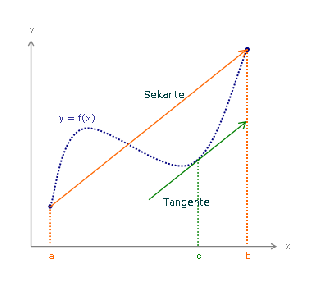
\epsfig{file=Figures/mean-value-theorem.eps,scale=1.5}
        \caption{Geometrische Bedeutung des Mittelwert-Satzes.}
        \label{fig:mean-value-theorem}
      \end{figure}


\begin{Satz}[Erweiterter Mittelwert-Satz]
  Sind die Funktion $f,g:[a,b] \rightarrow \mathbb{R}$ f\"ur alle $x\in[a,b]$
  differenzierbar und gilt $\df{g}(x) \not= 0$ f\"ur alle $x \in [a,b]$,
  so gilt: 
  \\[0.3cm]
  \hspace*{1.3cm}
  $\exists c \in (a,b): \bruch{f'(c)}{g'(c)} = \bruch{f(b) - f(a)}{g(b) - g(a)}$.
  \eox
\end{Satz}

\noindent
\textbf{Bemerkung}: Auf den ersten Blick mag es verwundern, dass nicht explizit 
$g(a) \not = g(b)$ gefordert wird.  Dies folgt aber sofort aus der Bedingung
$\forall x \in [a,b]:\df{g}(x) \not= 0$ und dem Satz von Rolle. \eox
\vspace*{0.3cm}

\exercise
Beweisen Sie den erweiterten Mittelwert-Satz.  Betrachten Sie dazu die Funktion
\\[0.2cm]
\hspace*{1.3cm}
$h(x) := \alpha \cdot f(x) - \beta \cdot g(x)$
\\[0.2cm]
und bestimmen Sie $\alpha$ und $\beta$ so, dass Sie auf die Funktion $h$ den Satz von Rolle anwenden k\"onnen. \eox
\vspace*{0.3cm}

% \solution
% Nach dem Mittelwert-Satz der Differential-Rechnung gibt es ein $c \in [a,b]$, so dass
% \\[0.2cm]
% \hspace*{1.3cm}
% $\ds \df{h}(c) = \frac{h(b) - h(a)}{b - a}$
% \\[0.2cm]
% gilt.  Wir berechnen die Werte von $h$, die in dieser Gleichung eine Rolle spielen, getrennt.
% \begin{enumerate}
% \item $h(a) = \bigl(g(b) - g(a) \bigr) \cdot f(a) - \bigl(f(b) - f(a)\bigr) \cdot g(a)$, 
% \item $h(b) = \bigl(g(b) - g(a) \bigr) \cdot f(b) - \bigl(f(b) - f(a)\bigr) \cdot g(b)$,
% \item $\df{h}(x) = \bigl(g(b) - g(a) \bigr) \cdot \df{f}(x) - \bigl(f(b) - f(a)\bigr) \cdot \df{g}(x)$.
% \end{enumerate}
% Damit finden wir
% \\[0.2cm]
% \hspace*{0.3cm}
% $
% \begin{array}[t]{lcrl}
% h(b) - h(a) & = &   & \bigl(g(b) - g(a) \bigr) \cdot f(b) - \bigl(f(b) - f(a)\bigr) \cdot g(b) \\[0.1cm]
%             &   & - & \bigl(g(b) - g(a) \bigr) \cdot f(a) + \bigl(f(b) - f(a)\bigr) \cdot g(a) \\[0.2cm]
%             & = &   & \bigl(g(b) - g(a) \bigr) \cdot \bigl(f(b) - f(a)\bigr) - \bigl(f(b) - f(a)\bigr) \cdot \bigl(g(b) - g(a) \bigr) \\[0.2cm]
%             & = &   & 0.
% \end{array}
% $
% \\[0.2cm]
% Nach dem Satz von Rolle finden wir also ein $c \in [a,b]$, so dass $\df{h}(c) = 0$ ist.  Setzen wir
% $c$ in die Formel f\"ur $\df{h}(x)$ ein, so erhalten wir
% \\[0.2cm]
% \hspace*{1.3cm}
% $0 = \bigl(g(b) - g(a) \bigr) \cdot \df{f}(c) - \bigl(f(b) - f(a)\bigr) \cdot \df{g}(c)$
% \\[0.2cm]
% Daraus folgt
% \\[0.2cm]
% \hspace*{1.3cm}
% $\ds \frac{f'(c)}{g'(c)} = \frac{f(b) - f(a)}{g(b) - g( a)}$ 
% \\[0.2cm]
% und das ist die Behauptung.
% \qed

Der folgende Satz ist f\"ur die praktische Berechnung von Grenzwerten unentbehrlich.  Wir haben
diesen Satz bereits mehrfach in der Vorlesung \"uber \emph{Algorithmen und Komplexit\"at} zur
Berechnung von Grenzwerten benutzt.

\begin{Satz}[Guillaume Fran\c{c}ois Antoine, Marquis de L'H\^opital, 1661--1704] \lb 
  Die Funktionen $f,g: (a,b) \rightarrow \mathbb{R}$ seien
  differenzierbar, es sei $c \in (a,b)$ und es gelte
  \begin{enumerate}
  \item $f(c) = g(c) = 0$ \quad und
  \item $\forall x \in (a,b):  g'(x) \not= 0$.
  \end{enumerate}
  Dann gilt 
  \\[0.3cm]
  \hspace*{1.3cm}
  $\lim\limits_{x \rightarrow c} \bruch{f(x)}{g(x)} = \bruch{f'(c)}{g'(c)}$.
\end{Satz}

\noindent
\textbf{Beweis}: 
Da die Funktion $f$ und $g$ im Punkt $c$ differenzierbar sind, gibt es Funktionen $r_1(h)$
und $r_2(h)$, so dass gilt:
\begin{enumerate}
\item $f(c+h) = f(c) + h\cdot f'(c) + r_1(h)$ \quad mit $\lim\limits_{h \rightarrow 0} \bruch{r_1(h)}{h} = 0$.
\item $g(c+h) = g(c) + h\cdot g'(c) + r_2(h)$ \quad mit $\lim\limits_{h \rightarrow 0} \bruch{r_2(h)}{h} = 0$.
\end{enumerate}
Wir haben die folgende Kette von Gleichungen:
\\[0.3cm]
\hspace*{1.3cm}
$
\begin{array}[b]{lclcl}
    \lim\limits_{h \rightarrow 0} \bruch{f(c+h)}{g(c+h)} &=&
    \lim\limits_{h \rightarrow 0} \bruch{f(c) + h\cdot f'(c) + r_1(h)}{g(c) + h\cdot g'(c) + r_2(h)} 
&=& \lim\limits_{h \rightarrow 0} \bruch{h\cdot f'(c) + r_1(h)}{h\cdot g'(c) + r_2(h)} \\[0.5cm]
&=& \lim\limits_{h \rightarrow 0} \bruch{f'(c) + \frac{r_1(h)}{h}}{g'(c) + \frac{r_2(h)}{h}} 
&=& \bruch{f'(c) + \lim\limits_{h \rightarrow 0} \frac{r_1(h)}{h}}{g'(c) + \lim\limits_{h \rightarrow 0} \frac{r_2(h)}{h}} \\[0.8cm]
&=& \bruch{f'(c)}{g'(c)} \\[0.5cm]
\end{array}
$
\hspace*{\fill} $\Box$


\example
Mit dem Satz von L'H\^opital k\"onnen wir nun den Grenzwert
$\ds\lim\limits_{x \rightarrow 0} \frac{\sin(x)}{x}$ noch einmal berechnen: 
\\[0.1cm]
\hspace*{1.3cm} $\ds\lim\limits_{x \rightarrow 0} \frac{\sin(x)}{x} = \lim\limits_{x \rightarrow 0}
\frac{\cos(x)}{1} = \cos(0) = 1$.
\\[0.2cm]
Sie sollten allerdings sehen, dass wir bei dieser Berechnung ausgenutzt haben, dass
\\[0.2cm]
\hspace*{1.3cm}
$\df{}\sin(x) = \cos(x)$
\\[0.2cm]
gilt und diese Gleichung konnten wir nur beweisen, weil wir vorher gezeigt hatten, dass
\\[0.2cm]
\hspace*{1.3cm}
$\ds\lim\limits_{x \rightarrow 0} \frac{\sin(x)}{x} = 1$
\\[0.2cm]
ist.
\eox

\remark
Der Satz von L'H\^opital beh\"alt seine G\"ultigkeit, wenn $x$ gegen Unendlich strebt.  Sind 
$f,g:\mathbb{R} \rightarrow \mathbb{R}$ differenzierbare Funktionen, so dass der Grenzwert
\\[0.3cm]
\hspace*{1.3cm}
$\ds\lim\limits_{x \rightarrow \infty} \frac{f'(x)}{g'(x)}$ 
\\[0.3cm]
existiert, und gilt entweder 
\\[0.3cm]
\hspace*{0.3cm}
$\Bigl(\lim\limits_{x \rightarrow \infty} f(x) = 0 \;\wedge\; \lim\limits_{x \rightarrow \infty} g(x) = 0\Bigr) \quad \vee \quad
 \Bigl(\lim\limits_{x \rightarrow \infty} f(x) = \infty \;\wedge\;\lim\limits_{x \rightarrow \infty} g(x) = \infty\Bigr)$ 
\\[0.3cm]
so folgt
\\
\hspace*{1.3cm}
$\ds\lim\limits_{x \rightarrow \infty} \frac{f(x)}{g(x)} = \lim\limits_{x \rightarrow \infty} \frac{f'(x)}{g'(x)}$.
\\[0.3cm]
Wir geben ein Beispiel.  Es gilt 
\\[0.3cm]
\hspace*{1.3cm}
$\ds\lim\limits_{x \rightarrow \infty} \frac{x}{\exp(x)} = \lim\limits_{x \rightarrow \infty} \frac{1}{\exp(x)} = 0$.
\\[0.3cm]
Wir haben es zwar nicht bewiesen, aber es kann gezeigt werden, dass der Satz von L'H\^opital  sich
auch iteriert anwenden l\"a{\ss}t.  Beispielsweise gilt
\\[0.3cm]
\hspace*{1.3cm}
$\ds\lim\limits_{x \rightarrow \infty} \frac{x^2}{\exp(x)} = \lim\limits_{x \rightarrow \infty}
\frac{2\cdot x}{\exp(x)} =\lim\limits_{x \rightarrow \infty} \frac{2}{\exp(x)} = 0$. \eox

\exercise
Berechnen Sie den Grenzwert \quad $\ds\lim\limits_{x \rightarrow 0} \frac{\cos(x) - 1}{x^2}$. \eox


\begin{Definition}[Schnelleres Wachstum] \lb
  Wir sagen, dass die Funktion $x \mapsto f(x)$ f\"ur $x \rightarrow \infty$ \emph{schneller als} die
  Funktion $x \mapsto g(x)$ \emph{w\"achst}, falls 
  \\[0.2cm]
  \hspace*{1.3cm}
  $\ds \lim\limits_{x \rightarrow \infty} \frac{g(x)}{f(x)} = 0$
  \\[0.2cm]
  gilt. \eox
\end{Definition}

\exercise
Zeigen Sie, dass f\"ur alle nat\"urlichen Zahlen $n$ gilt: 
\\[0.3cm]
\hspace*{1.3cm} $\lim\limits_{x \rightarrow \infty} \bruch{x^n}{\exp(x)} = 0$.
\\[0.3cm]
Damit sehen wir, dass die Exponential-Funktion schneller w\"achst als jede Potenz.  
\eox

\exercise
\begin{enumerate}[(a)]
\item Zeigen Sie, dass die Funktion $\ds x \mapsto \exp\bigl(\ln(x) \cdot \ln(x)\bigr)$ f\"ur alle $n \in \mathbb{N}$ schneller
      als die Funktion $x \mapsto x^n$ w\"achst.
\item Zeigen Sie, dass die Funktion $\ds x \mapsto \exp(x)$ schneller w\"achst als die Funktion
      $\ds x \mapsto \exp\bigl(\ln(x) \cdot \ln(x)\bigr)$. \eox
\end{enumerate} 

\exercise
Berechnen Sie die folgenden Grenzwerte:
\begin{enumerate}[(a)]
\item $\ds\lim\limits_{x \rightarrow 0} x \cdot \ln(x)$,
\item $\ds\lim\limits_{x \rightarrow \infty} \sqrt{x + \sqrt{x\;}\;} - \sqrt{x\;}$.  \eox
\end{enumerate}

\section{Monotonie und Konvexit\"at}
Im Folgenden bezeichnet $D$ entweder ein
\href{http://de.wikipedia.org/wiki/Intervall_(Mathematik)}{Intervall} der Form
\\[0.2cm]
\hspace*{1.3cm}
$[a, b]$, \quad  
$(a, b]$, \quad   
$[a, b)$, \quad    
$(a, b)$,
\\[0.2cm]
ein unbeschr\"anktes Intervall der Form
\\[0.2cm]
\hspace*{1.3cm}
$[a, \infty)$, \quad      
$(a, \infty)$, \quad       
$(-\infty, b]$, \quad        
$(-\infty, b)$ \quad        
\\[0.2cm]
oder die Menge $\mathbb{R}$ der reellen Zahlen.

\begin{Definition}[monoton]
  Eine Funktion $f: D \rightarrow \mathbb{R}$ ist \colorbox{orange}{\emph{monoton steigend}} g.d.w.
  \\[0.2cm]
  \hspace*{1.3cm}
  $\forall x,y \in D:\bigl(x < y \rightarrow f(x) \leq f(y)\bigr)$
  \\[0.2cm]
  gilt.  Die Funktion $f$ ist \colorbox{orange}{\emph{streng monoton steigend}}, wenn die sch\"arfere Bedingung
  \\[0.2cm]
  \hspace*{1.3cm}
  $\forall x,y \in D:\bigl(x < y \rightarrow f(x) < f(y)\bigr)$
  \\[0.2cm]
  erf\"ullt ist.  Weiter hei{\ss}t  $f$ \colorbox{orange}{\emph{monoton fallend}}, wenn
  \\[0.2cm]
  \hspace*{1.3cm}
  $\forall x,y \in D:\bigl(x < y \rightarrow f(x) \geq f(y)\bigr)$
  \\[0.2cm]
  gilt.  Analog ist $f$ \colorbox{orange}{\emph{streng monoton fallend}}, falls die folgende Bedingung gilt:
  \\[0.2cm]
  \hspace*{1.3cm}
  $\forall x,y \in D:\bigl(x < y \rightarrow f(x) > f(y)\bigr)$.
  \eod
\end{Definition}

\begin{Satz} \label{satz:monoton}
  Eine differenzierbare Funktion $f:D \rightarrow \mathbb{R}$ ist genau dann
  monoton steigend, wenn gilt: 
  \\[0.2cm]
  \hspace*{1.3cm} $\forall x \in D: f'(x) \geq 0$.
  \eod
\end{Satz}


\noindent
\textbf{Beweis}: Da es sich bei diesem Beweis um eine "genau-dann-wenn"-Aussage handelt, spalten wir
den Beweis in zwei Teile auf.
\begin{enumerate}
\item[``$\Rightarrow$'':]  Wir nehmen zun\"achst an, dass $f$ monoton steigend ist und zeigen, dass
      dann $f'(x) \geq 0$ gilt.  Die Ableitung ist definiert als der Grenzwert 
      \\[0.3cm]
      \hspace*{1.3cm} $f'(x) = \lim\limits_{h \rightarrow 0} \bruch{f(x+h) - f(x)}{h}$.
      \\[0.3cm]
      Wir zeigen, dass der Differential-Quotient 
      \\[0.3cm]
      \hspace*{1.3cm} $\bruch{f(x+h) - f(x)}{h}$
      \\[0.3cm]
      f\"ur alle $h \not = 0$ gr\"o{\ss}er oder gleich 0 ist.  Zum Nachweis dieser Behauptung f\"uhren wir
      eine Fallunterscheidung bez\"uglich des Vorzeichens von $h$ durch.
      \begin{enumerate}[(a)]
      \item Fall: $h > 0$.
        
            Aus $h > 0$ folgt $x + h > x$.  Aus der Monotonie von $f$ folgt dann,  dass 
            $f(x+h) \geq f(x)$ ist.  Also gilt $f(x+h)-f(x) \geq 0$ und daraus folgt
            \\[0.3cm]
            \hspace*{1.3cm} $\bruch{f(x+h) - f(x)}{h} \geq 0$.
      \item Fall: $h < 0$.
        
            Aus $h < 0$ folgt nun $x + h < x$.
            Aus der Monotonie von $f$ folgt jetzt die Ungleichung 
            $f(x+h) \leq f(x)$.  Also haben wir  $f(x+h)-f(x) \leq 0$.  Wegen $h<0$ gilt dann
            insgesamt
            \\[0.3cm]
            \hspace*{1.3cm} $\bruch{f(x+h) - f(x)}{h} \geq 0$.
      \end{enumerate}
      Da der Differential-Quotient in jedem Fall gr\"o{\ss}er-gleich $0$ ist und die Ableitung $f'(x)$ als
      Grenzwert des Differential-Quotienten f\"ur $h$ gegen $0$ definiert ist, muss $f'(x) \geq 0$
      gelten.
\item[``$\Leftarrow$'':] Wir nehmen nun an, dass f\"ur alle $x\in D$ die Ungleichung $f'(x) \geq 0$ gilt und
      zeigen, dass $f$ dann monoton steigend ist.  Diesen Beweis f\"uhren wir indirekt.
      Wir nehmen an, es g\"abe $x,y\in D$ mit 
      \\[0.2cm]
      \hspace*{1.3cm} $x < y$ \quad aber \quad $f(x) > f(y)$.
      \\[0.2cm]
      Nach dem Mittelwert-Satz der Differential-Rechnung gibt es dann ein $z\in[x,y]$, so dass
      \\[0.3cm]
      \hspace*{1.3cm} $f'(z) = \bruch{f(y) - f(x)}{y - x}$
      \\[0.3cm]
      gilt.  Aus $x < y$ folgt  $y - x \geq 0$ und aus $f(x) > f(y)$ folgt $f(y) - f(x) <0$.
      Damit h\"atten wir dann aber $f'(z) < 0$ im Widerspruch zur Voraussetzung.
      \qed
\end{enumerate} 
\vspace*{0.1cm}

\noindent
In Analogie zum letzten Satz kann gezeigt werden, dass eine differenzierbare Funktion 
$f:D \rightarrow \mathbb{R}$ genau dann monoton
fallend ist, wenn f\"ur alle $x\in D$ die Ungleichung $f'(x) \leq 0$ gilt.

\exercise
Die Funktion $f:D \rightarrow \mathbb{R}$ sei differenzierbar und es gelte
\\[0.2cm]
\hspace*{1.3cm}
$\forall x \in D: f'(x) > 0$.
\\[0.2cm]
Zeigen Sie, dass die Funktion $f$ dann \underline{stren}g monoton steigend ist.
\vspace*{0.3cm}

\noindent
\textbf{Bemerkung:}
Die Funktion $x \mapsto x^3$ ist streng monoton steigend, aber an der Stelle $x=0$
verschwindet die Ableitung dieser Funktion.  Dies zeigt, dass sich die Aussage des letzten
Satzes nicht umkehren l\"asst. \eox


\begin{Definition}[strenges lokales Minimum] \lb
  Eine Funktion $f:\mathbb{R} \rightarrow \mathbb{R}$ hat im Punkt $\bar{x}\in \mathbb{R}$
  ein \colorbox{orange}{\emph{strenges lokales Minimum}}, wenn gilt:
  \\[0.2cm]
  \hspace*{1.3cm}
  $\exists \varepsilon \in \mathbb{R}_+: \forall x \in \mathbb{R}:\bigl( 
  |x - \bar{x}| < \varepsilon \wedge\ x \not= \bar{x} \rightarrow f(x) > f(\bar{x})\bigr)$.
\eod
\end{Definition}

\noindent
\textbf{Bemerkung}:  Der Begriff des \colorbox{orange}{\emph{strengen lokalen Maximum}} l\"asst sich
analog definieren. 

\begin{Satz} \label{satz:minimum}
  Die Funktion $f:\mathbb{R} \rightarrow \mathbb{R}$ sei zweimal differenzierbar, die
  zweite Ableitung $f''(x)$ sei stetig und f\"ur
  ein $x_0 \in \mathbb{R}$ gelte
  \\[0.2cm]
  \hspace*{1.3cm}
  $f'(x_0) = 0 \;\wedge\; f''(x_0) > 0$.
  \\[0.2cm]
  Dann hat die Funktion $f$ im Punkt $x_0$ ein strenges lokales Minimum.
\end{Satz}

\proof Da die zweite Ableitung $f''(x)$ stetig ist, k\"onnen wir $\varepsilon := f''(x_0) > 0$
setzen und finden dann ein $\delta > 0$, so dass
\\[0.2cm]
\hspace*{1.3cm}
 $\forall x \in \mathbb{R}:\bigl(
    |x - x_0| < \delta \rightarrow |f''(x) - f''(x_0)| < \varepsilon = f''(x_0)\bigr)
$.
\\[0.2cm]
gilt.  Subtrahieren wir $|f''(x) - f''(x_0)|$ auf beiden Seiten dieser Gleichung, so folgt, dass f\"ur
alle $x \in \mathbb{R}$ mit $|x - x_0| < \delta$ die Ungleichung
\\[0.2cm]
\hspace*{1.3cm} $f''(x_0) - |f''(x) - f''(x_0)| > 0$
\\[0.2cm]
gilt.  Wir behaupten, dass dann
\begin{equation}
  \label{eq:minimum}
 f''(x) > 0 \quad \mbox{f\"ur alle $x \in \mathbb{R}$ mit $|x - x_0| < \delta$} 
\end{equation}
gilt.
Zum Nachweis dieser Behauptung f\"uhren wir eine Fallunterscheidung bez\"uglich der relativen
Gr\"o{\ss}e von $f''(x)$ und $f''(x_0)$ durch.
\begin{enumerate}
\item Fall: $f''(x) < f''(x_0)$.  Dann gilt 
      \\[0.2cm]
      \hspace*{1.3cm}
      $|f''(x) - f''(x_0)| = f''(x_0) - f''(x)$.
      \\[0.2cm]
      Also folgt aus der Ungleichung $f''(x_0) - |f''(x) - f''(x_0)| > 0$ die Ungleichung
      \\[0.2cm]
      \hspace*{1.3cm}
      $f''(x_0) - \bigl(f''(x_0) - f''(x)\bigr) > 0$
      \\[0.2cm]
      und wegen $f''(x_0) - \bigl(f''(x_0) - f''(x)\bigr) = f''(x)$ haben wir damit die Behauptung
      $f''(x) > 0$ gezeigt.
\item Fall: $f''(x) \geq f''(x_0)$.  

      In diesem Fall folgt die Behauptung sofort aus der Voraussetzung
      $f''(x_0) > 0$ und der Transitivit\"at der Relation $>$.
\end{enumerate}
Zusammen mit dem Satz \ref{satz:monoton} zeigt die Ungleichung (\ref{eq:minimum}), dass die Funktion
$x \mapsto f'(x)$ in der $\delta$-Umgebung von $x_0$ streng monoton steigend ist.  Da au{\ss}erdem
$f'(x_0) = 0$ gilt, folgt insgesamt 
\\[0.2cm]
\hspace*{1.3cm}
$f'(x) < 0$ \quad f\"ur alle $x\in U_\delta(x_0)$ mit $x < x_0$ \quad und \quad \\[0.2cm]
\hspace*{1.3cm}
$f'(x) > 0$ \quad f\"ur alle $x\in U_\delta(x_0)$ mit $x > x_0$.
\\[0.2cm]
Damit ist die Funktion $f$ innerhalb der $\delta$-Umgebung $U_\delta(x_0)$ f\"ur $x < x_0$
streng monoton fallend und f\"ur $x > x_0$ streng monoton wachsend.  Dann muss $f$ aber ein lokales
Minimum im Punkt $x_0$ haben. \qed


\noindent
\textbf{Bemerkung}: Falls f\"ur die Funktion $f$ die Bedingung
\\[0.2cm]
\hspace*{1.3cm}
$f'(x_0) = 0 \wedge f''(x_0) < 0$.
\\[0.2cm]
erf\"ullt ist, dann hat die Funktion an der Stelle $x_0$ ein strenges lokales Maximum. \eox


\begin{Definition}[konvex, konkav]
Eine Funktion $f:\mathbb{R} \rightarrow \mathbb{R}$ hei{\ss}t \colorbox{orange}{\emph{konvex}} genau dann, wenn 
\\[0.2cm]
\hspace*{1.3cm}
$\forall x_1,x_2 \in \mathbb{R}:\forall t\in [0,1]: \bigl(
  f\bigl(t \cdot x_1 + (1-t)\cdot x_2\bigr) \leq t \cdot f(x_1) + (1 - t) \cdot f(x_2)
  \bigr)
$
\\[0.2cm]
gilt.  Geometrisch bedeutet dies, dass die Funktionswerte der Funktion $f$  unterhalb
der Sekante durch die Punkte 
$\bigl\langle x_1, f(x_1) \bigl\rangle$ und $\bigl\langle x_2, f(x_2) \bigl\rangle$
liegen.  Abbildung \ref{fig:convex.eps} auf Seite \pageref{fig:convex.eps} zeigt dies anschaulich: 
In dem Intervall $(x_1,x_2)$ liegen die Werte der Funktion $f$ unterhalb der Gerade $g$, die durch die beiden Punkte 
$\langle x_1, f(x_1)\rangle$ und $\langle x_2, f(x_2)\rangle$ geht.  Die Gleichung dieser Geraden
ist 
\\[0.2cm]
\hspace*{1.3cm}
$\ds g(x) = \frac{x-x_1}{x_2-x_1}\cdot f(x_2) + \frac{x-x_2}{x_1-x_2}\cdot f(x_1)$.
\\[0.2cm]
Sie k\"onnen dies sofort verifizieren, denn offenbar ist $g(x)$ in der Variablen $x$ linear und
andererseits gilt
\\[0.2cm]
\hspace*{1.3cm}
$\ds g(x_1) = \frac{x_1-x_1}{x_2-x_1}\cdot f(x_2)+\frac{x_1-x_2}{x_1-x_2}\cdot f(x_1) = f(x_1)$
\\[0.2cm]
und analog sehen wir, dass auch $g(x_2) = f(x_2)$ ist.  Die Tatsache, dass $f(x)$ f\"ur $x \in [x_1,x_2]$
unterhalb der Geraden $g(x)$ liegt, bedeutet, dass
\\[0.2cm]
\hspace*{1.3cm}
$f(x) \leq g(x)$  \quad f\"ur alle $x \in [x_1,x_2]$
\\[0.2cm]
gilt.  Jedes $x \in [x_1,x_2]$ l\"asst sich in der Form
\\[0.2cm]
\hspace*{1.3cm}
$x = t \cdot x_1 + (1-t) \cdot x_2$
\\[0.2cm]
schreiben, wobei $t \in [0,1]$ gilt.  Setzen wir diesen Wert von $x$ in die Ungleichung $f(x) \leq g(x)$
ein, so erhalten wir 
\\[0.2cm]
\hspace*{1.3cm}
$
\begin{array}[t]{cl}
      &  f\bigl(t \cdot x_1 + (1-t) \cdot x_2)\bigr) \\[0.2cm]
 \leq & g\bigl(t \cdot x_1 + (1-t) \cdot x_2)\bigr)  \\[0.2cm]
  =   & \ds \frac{\bigl(t \cdot x_1 + (1-t) \cdot x_2\bigr) - x_1}{x_2-x_1} \cdot f(x_2) + 
            \frac{\bigl(t \cdot x_1 + (1-t) \cdot x_2\bigr) - x_2}{x_1-x_1} \cdot f(x_1) 
        \\[0.4cm]
  =   & \ds \frac{(1-t) \cdot x_2 - (1-t) \cdot x_1}{x_2-x_1} \cdot f(x_2) + 
            \frac{t \cdot x_1 - t \cdot x_2}{x_1-x_1} \cdot f(x_1) 
        \\[0.4cm]
  =   & \ds (1-t) \cdot f(x_2) + t \cdot f(x_1) 
\end{array}
$
\\[0.2cm]
und das ist genau die Definition der Konvexit\"at.
\vspace*{0.2cm}

Eine Funktion $f:\mathbb{R} \rightarrow \mathbb{R}$ hei{\ss}t \colorbox{orange}{\emph{konkav}} genau dann, wenn 
\\[0.2cm]
\hspace*{1.3cm}
$\forall x_1,x_2 \in \mathbb{R}:\forall t\in [0,1]: 
  f\bigl(t \cdot x_1 + (1-t)\cdot x_2\bigr) \geq t \cdot f(x_1) + (1 - t) \cdot f(x_2)
$
\\[0.2cm]
gilt.  Hier liegen die Funktionswerte der Funktion $f$ also oberhalb 
der Sekante durch die Punkte 
$\bigl\langle x_1, f(x_1) \bigl\rangle$ und $\bigl\langle x_2, f(x_2) \bigl\rangle$.
\\[0.2cm]
Abbildung \ref{fig:concav.eps} auf Seite \pageref{fig:concav.eps} zeigt eine konkave Funktion $f$
zusammen mit einer Sekante $g$.  
\eod
\end{Definition}

\begin{figure}[!h]
  \centering
    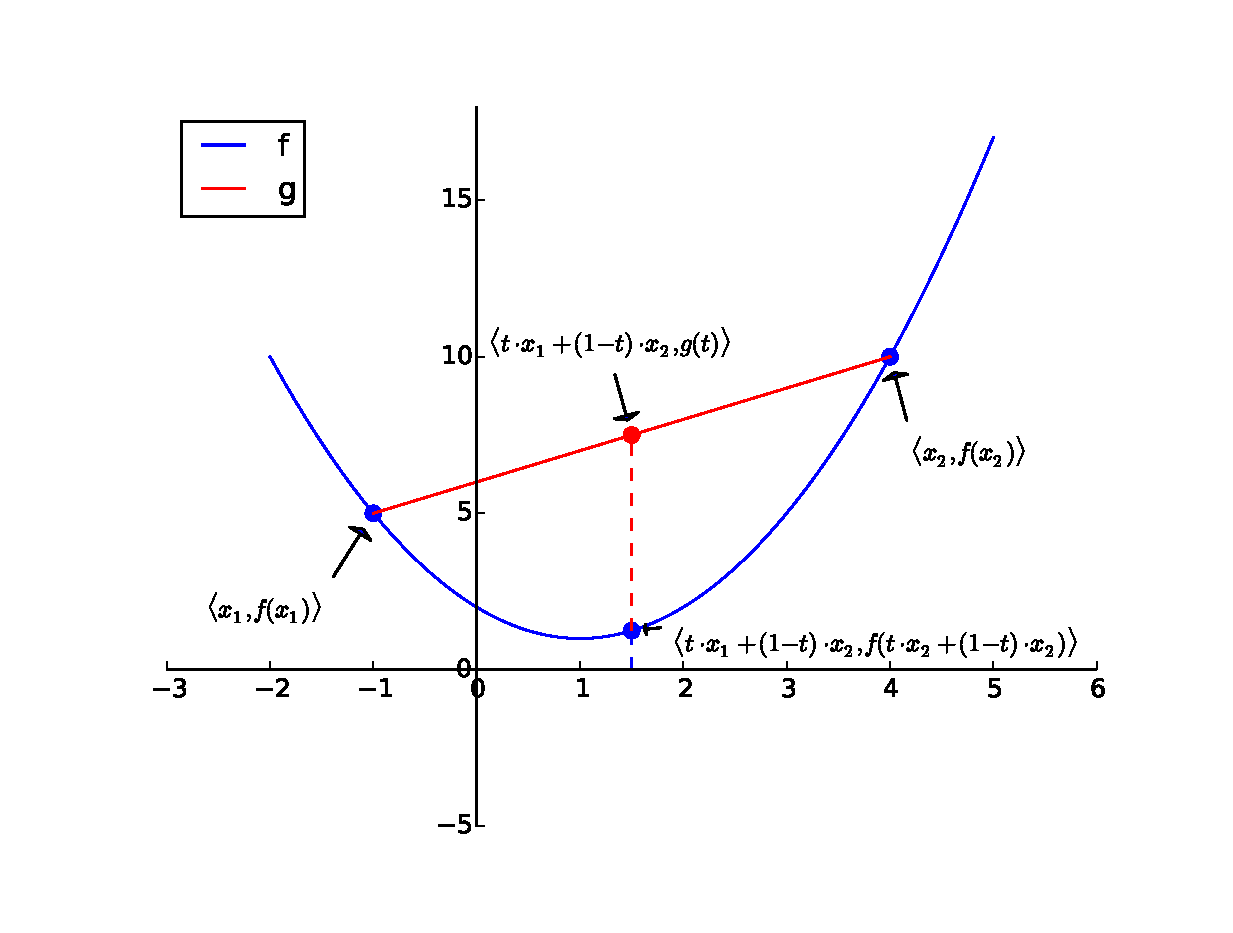
\epsfig{file=Figures/convex.eps,scale=0.6}
   \caption{Eine konvexe Funktion $f$ zusammen mit einer Sekante $g$.}
  \label{fig:convex.eps}
\end{figure}
\begin{figure}[!h]
  \centering
    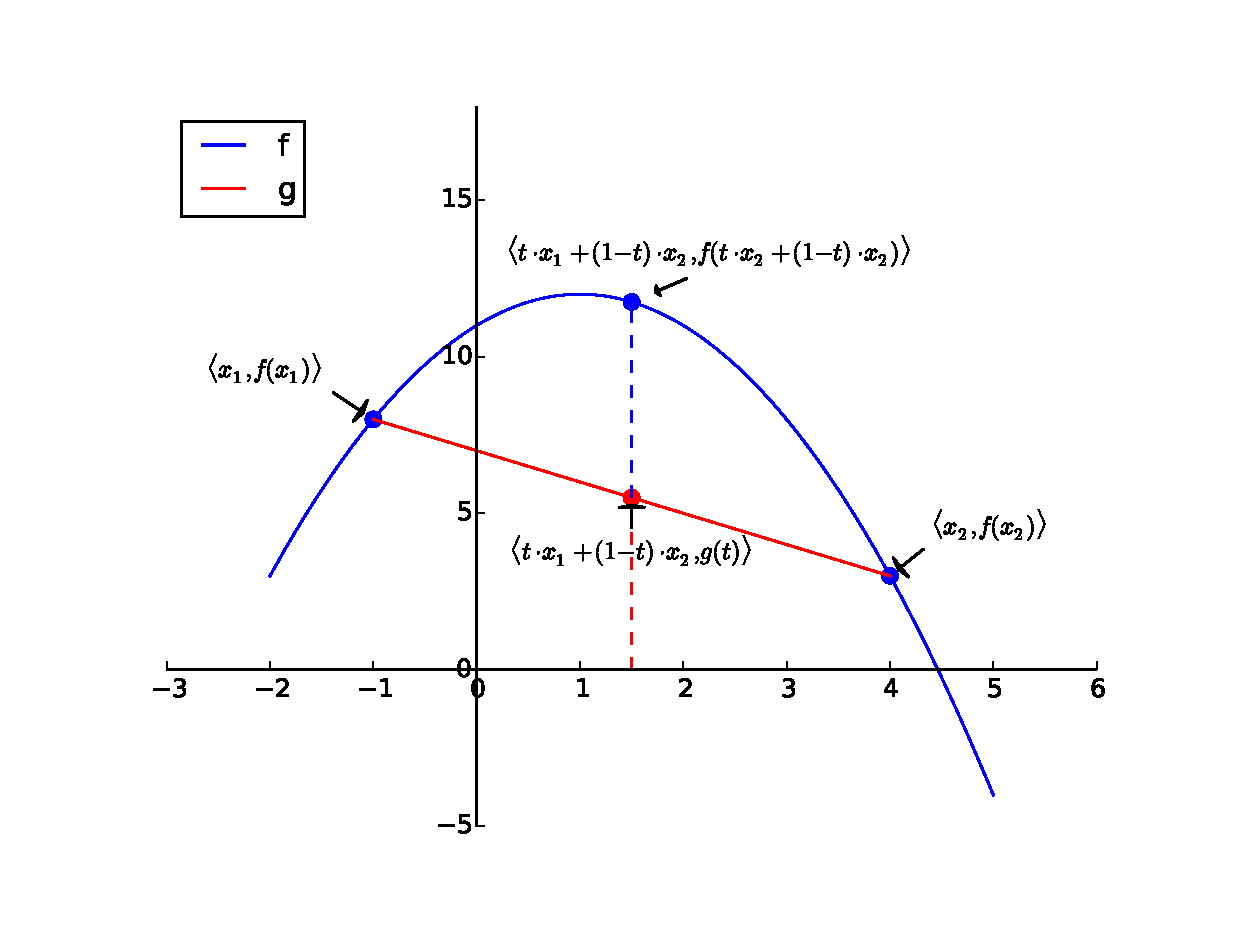
\epsfig{file=Figures/concav.eps,scale=0.6}
   \caption{Eine konkave Funktion $f$ zusammen mit einer Sekante $g$.}
  \label{fig:concav.eps}
\end{figure}




\begin{Lemma}[Invarianz der Konvexit\"at unter linearen Transformationen]
  \label{lemma:konvex_invarianz} \lb
  Die Funktion $f:\mathbb{R} \rightarrow \mathbb{R}$ sei konvex und es seien $\alpha, \beta \in \mathbb{R}$.
  Definieren wir die Funktion $g:\mathbb{R} \rightarrow \mathbb{R}$ als
  \\[0.2cm]
  \hspace*{1.3cm}
  $g(x) := f(x) + \alpha \cdot x + \beta$,
  \\[0.2cm]
  so ist auch die Funktion $g$ konvex.  Eine entsprechende Aussage gilt auch f\"ur konkave Funktionen.
\end{Lemma}

\exercise
Beweisen Sie das vorangehende Lemma. \eox
\pagebreak

\begin{Satz}
Die Funktion $f:\mathbb{R} \rightarrow \mathbb{R}$ sei zweimal differenzierbar und die Funktion 
$x \mapsto f''(x)$ sei stetig.  Dann gilt 
\\[0.2cm]
\hspace*{1.3cm}
$f$  konvex \quad $\Leftrightarrow$ \quad $\forall x \in \mathbb{R}: f''(x) \geq 0$.
\end{Satz}

\noindent
\textbf{Beweis}: Wir spalten den Beweis in zwei Teile auf.
\begin{enumerate}
\item[``$\Rightarrow$'':] Wir f\"uhren den Nachweis indirekt und nehmen an, dass es ein $x_0 \in \mathbb{R}$
  gibt, so dass $f''(x_0) < 0$ ist.  \"Ahnlich wie im Beweis von Satz \ref{satz:minimum} folgt daraus, dass
  es eine $\delta_1$-Umgebung $U_{\delta_1}(x_0)$ gibt, so dass
  \\[0.2cm]
  \hspace*{1.3cm} $f''(x) < 0$ \quad f\"ur alle $x \in U_{\delta_1}(x_0)$ 
  \\[0.2cm]
  gilt.  Wir definieren eine Funktion $g:\mathbb{R} \rightarrow \mathbb{R}$ durch
  \\[0.2cm]
  \hspace*{1.3cm}
  $g(x) := f(x) - x \cdot f'(x_0)$.
  \\[0.2cm]
  Dann gilt 
  \\[0.2cm]
  \hspace*{1.3cm}
  $g'(x) = f'(x) - f'(x_0)$ \quad und \quad $g''(x) = f''(x)$.
  \\[0.2cm]
  Daraus folgt durch Einsetzen
  \\[0.2cm]
  \hspace*{1.3cm}
  $g'(x_0) = 0$ \quad und \quad $g''(x_0) < 0$.
  \\[0.2cm]
  Damit hat die Funktion $g$ im Punkt $x_0$ ein lokales Maximum.  Also gibt es eine $\delta_2$-Umgebung von
  $x_0$, so dass
  \\[0.2cm]
  \hspace*{1.3cm}
  $g(x) < g(x_0)$ \quad f\"ur alle $x \in U_{\delta_2}(x_0)$
  \\[0.2cm]
  gilt.  O.B.d.A. k\"onnen wir voraussetzen, dass $\delta_2 \leq \delta_1$ gilt.  
  Nach dem Lemma \ref{lemma:konvex_invarianz} wissen wir, dass die Funktion $g$ ebenfalls konvex ist.
  Definieren wir
\\[0.2cm]
\hspace*{1.3cm}
 $\ds x_1 := x_0 - \frac{\delta_2}{2}$, \quad $\ds x_2 := x_0 + \frac{\delta_2}{2}$ \quad und \quad $\ds t := \frac{1}{2}$,
\\[0.2cm]
  so folgt also
  \begin{equation}
    \label{eq:konvex1}
  t \cdot g(x_1) + (1 - t) \cdot g(x_2) \geq g\bigl(t \cdot x_1 + (1-t) \cdot x_2\bigr).
  \end{equation}
  Nun gilt 
  \\[-0.2cm]
  \hspace*{1.3cm}
  $\ds t \cdot x_1 + (1-t) \cdot x_2 = 
   \frac{1}{2} \cdot x_0 - \frac{1}{2} \cdot\frac{\delta_2}{2} + 
   \frac{1}{2} \cdot x_0 + \frac{1}{2} \cdot\frac{\delta_2}{2}
   = x_0
  $.
  \\[0.2cm]
  Damit folgt aus der Ungleichung (\ref{eq:konvex1}) die Ungleichung
  \begin{equation}
    \label{eq:konvex2}    
  \frac{1}{2} \cdot g(x_1) + \frac{1}{2} \cdot g(x_2) \geq g(x_0).
  \end{equation} 
  Andererseits folgt aus der Tatsache, dass sowohl $x_1$ als auch $x_2$ in der $\delta_1$-Umgebung von $x_0$
  liegen, dass
  \\[0.2cm]
  \hspace*{1.3cm}
  $g(x_1) < g(x_0)$ \quad und \quad  $g(x_2) < g(x_0)$
  \\[0.2cm]
  gilt. Multiplizieren wir diese beiden Gleichungen mit $\frac{1}{2}$ und addieren sie, so ergibt sich
  \\[0.2cm]
  \hspace*{1.3cm}
  $\frac{1}{2} \cdot g(x_1) + \frac{1}{2} \cdot g(x_2) < g(x_0)$ .
  \\[0.2cm]
  Diese Ungleichung steht aber im Widerspruch zur Ungleichung (\ref{eq:konvex2}).
\item[``$\Leftarrow$'':]  Es seien $x_1$, $x_2$ und $t \in [0,1]$ gegeben.  O.B.d.A. sei weiter
  $x_1 < x_2$. Wir definieren zun\"achst
  \\[0.2cm]
  \hspace*{1.3cm}
  $x_0 := t \cdot x_1 + (1 - t) \cdot x_2$
  \\[0.2cm]
  Es l\"asst sich sofort nachrechnen, dass dann $x_1 < x_0 < x_2$ gilt.  Nach dem Mittelwert-Satz der
  Differential-Rechnung gibt es jeweils ein $c_1 \in [x_1,x_0]$ und ein $c_2 \in [x_0,x_2]$, so dass
  \\[0.2cm]
  \hspace*{1.3cm}
  $f'(c_1) = \bruch{f(x_0) - f(x_1)}{x_0 - x_1}$  \quad und \quad
  $f'(c_2) = \bruch{f(x_2) - f(x_0)}{x_2 - x_0}$  
  \\[0.2cm]
  gilt.  Da $f''(x) \geq 0$ ist, wissen wir au{\ss}erdem, dass die Funktion $f'(x)$ monoton steigend ist.
  Da offenbar $c_1 \leq c_2$ ist, folgt daraus die Ungleichung $f'(c_1) \leq f'(c_2)$ und damit gilt
  \begin{equation}
    \label{eq:konvex3}
    \bruch{f(x_0) - f(x_1)}{x_0 - x_1} \leq \bruch{f(x_2) - f(x_0)}{x_2 - x_0}.    
  \end{equation}
  Es gilt
  \\[-0.2cm]
  \hspace*{1.3cm}
  $x_0 - x_1 = t \cdot x_1 + (1 - t) \cdot x_2 - x_1 = (1-t) \cdot (x_2 - x_1)$
  \\[0.2cm]
  und genauso sehen wir
  \\[0.2cm]
  \hspace*{1.3cm}
  $x_2 - x_0 = x_2 - \bigl(t \cdot x_1 + (1 - t) \cdot x_2\bigr) = t \cdot (x_2 - x_1)$.
  \\[0.2cm]
  Multiplizieren wir daher die Ungleichung (\ref{eq:konvex3}) mit $t \cdot (1 - t) \cdot (x_2 -x_1)$, so
  erhalten wir die Ungleichung
  \\[0.2cm]
  \hspace*{1.3cm}
  $t \cdot \bigl(f(x_0) - f(x_1)\bigr) \leq (1 - t) \cdot \bigl(f(x_2) - f(x_0)\bigr)$.
  \\[0.2cm]
  Addieren wir auf beiden Seiten der Gleichung $(1 - t) \cdot f(x_0)$ und $t \cdot f(x_1)$
  und setzen dann noch f\"ur $x_0$ den Wert $t \cdot x_1 + (1-t)\cdot x_2$ ein, so erhalten wir
  die Ungleichung
  \\[0.2cm]
  \hspace*{1.3cm}
  $f\bigl(t \cdot x_1 + (1-t)\cdot x_2) \leq t \cdot f(x_1) + (1-t) \cdot f(x_2)$.
  \\[0.2cm]
  Das ist aber gerade die Konvexit\"at der Funktion $f$. \qed
\end{enumerate}
\pagebreak

\section{Die Exponential-Funktion}
Wir haben die Exponential-Funktion als die Potenzreihe
\\[0.2cm]
\hspace*{1.3cm}
$\ds\exp(x) := \sum\limits_{n=0}^\infty \bruch{1}{n!} \cdot x^{n}$ 
\\[0.2cm]
definiert und gesehen, dass diese Potenzreihe f\"ur alle $x \in \mathbb{R}$ konvergiert.
Wir definieren nun die Eulersche Zahl $\mathrm{e}$ (\href{http://de.wikipedia.org/wiki/Leonhard_Euler}{Leonhard Euler},
1707--1783) mit Hilfe der Exponential-Funktion als
\\[0.2cm]
\hspace*{1.3cm}
$\mathrm{e} := \exp(1) = \sum\limits_{n=0}^\infty \bruch{1}{n!} = 
  2.718\,281\,828\,459\,045\,235\,360\,287\,471\,352\,662\,497\,757\,247\,093\,\cdots
$.
\\[0.2cm]
Wir wollen in diesem Abschnitt zeigen, dass f\"ur die Exponential-Funktion die Gleichung 
\\[0.2cm]
\hspace*{1.3cm}
$\exp(x) = \mathrm{e}^x$ \quad 
\\[0.2cm]
gilt.  Zum Nachweis der oben behaupteten Gleichung ben\"otigen wir das folgende Lemma.

\begin{Lemma} \label{lemma:0_ableitung}
Ist die Funktion $f:\mathbb{R} \rightarrow \mathbb{R}$ f\"ur alle $x \in \mathbb{R}$
differenzierbar und gilt
\\[0.2cm]
\hspace*{1.3cm}
$f'(x) = 0$ \quad f\"ur alle $x \in \mathbb{R}$
\\[0.2cm]
so ist die Funktion $f$ konstant:  Es gibt dann ein $c \in \mathbb{R}$ so dass
\\[0.2cm]
\hspace*{1.3cm}
$f(x) = c$ \quad f\"ur alle $x \in \mathbb{R}$ ist.
\end{Lemma}

\proof
Wir betrachten zwei beliebige Zahlen $x_1, x_2\in \mathbb{R}$, f\"ur die
\\[0.2cm]
\hspace*{1.3cm}
$x_1 \not= x_2$ 
\\[0.2cm]
gilt.  O.B.d.A. sei $x_1 < x_2$.  Wir zeigen, dass dann 
\\[0.2cm]
\hspace*{1.3cm}
$f(x_1) = f(x_2)$
\\[0.2cm]
gilt.  Nach dem Mittelwert-Satz gibt es ein $c \in [x_1,x_2]$, so dass
\\[0.2cm]
\hspace*{1.3cm}
$f'(c) = \bruch{f(x_2) - f(x_1)}{x_2 - x_1}$ 
\\[0.2cm]
gilt.  Nach Voraussetzung wissen wir, dass $f'(c) = 0$ ist.  Also haben wir
\\[0.2cm]
\hspace*{1.3cm}
$0 = \bruch{f(x_2) - f(x_1)}{x_2 - x_1}$.
\\[0.2cm]
Multiplikation dieser Gleichung mit $x_2 - x_1$ liefert die Gleichung
\\[0.2cm]
\hspace*{1.3cm}
$0 = f(x_2) - f(x_1)$
\\[0.2cm]
und daraus folgt sofort $f(x_1) = f(x_2)$.  Damit ist gezeigt, dass die Funktion $f$ f\"ur alle
Argumente den selben Wert liefert und also konstant ist. \qed

\exercise
Zeigen Sie: Ist die Funktion $f:\mathbb{R} \rightarrow \mathbb{R}$ zweimal differenzierbar und gilt
$f''(x) = 0$ f\"ur alle $x \in \mathbb{R}$, so gibt es Zahlen $c,d \in \mathbb{R}$, so dass 
\\[0.2cm]
\hspace*{1.3cm}
$\forall x \in \mathbb{R}: f(x) = c \cdot x + d$
\\[0.2cm]
gilt.  \"Uberlegen  Sie, wie Sie diese Aussage so verallgemeinern k\"onnen, dass die verallgemeinerte Aussage
f\"ur beliebige $n$-mal differenzierbare 
Funktionen $f:\mathbb{R} \rightarrow \mathbb{R}$ gilt, f\"ur deren $n$-te Ableitung 
\\[0.2cm]
\hspace*{1.3cm}
$f^{(n)}(x) = 0$ \quad f\"ur alle $x \in \mathbb{R}$ ist.  \eox


\exercise
Zeigen Sie, dass f\"ur alle $x\in \mathbb{R}$
\\[0.2cm]
\hspace*{1.3cm}
$\exp(x) \cdot \exp(-x) = 1$ 
\\[0.2cm]
gilt.  Bei Ihrem Beweis sollen Sie die Gleichung $\exp(x+y) = \exp(x) \cdot \exp(y)$ nicht benutzen!
Folgern Sie aus der von Ihnen gezeigten Gleichung, dass die Exponential-Funktion keine Nullstelle hat. \eox
\vspace*{0.3cm}

\noindent
Aus dem letzten Lemma folgt eine wichtige Charakterisierung der Exponential-Funktion.
\begin{Lemma}
Die Funktion $f:\mathbb{R} \rightarrow \mathbb{R}$ sei f\"ur alle $x \in \mathbb{R}$ differenzierbar und es
gelte
\\[0.2cm]
\hspace*{1.3cm}
$f'(x) = \lambda \cdot f(x)$ \quad f\"ur ein $\lambda \in \mathbb{R}$.
\\[0.2cm]
Dann gibt es ein $c \in \mathbb{R}$, so dass
\\[0.2cm]
\hspace*{1.3cm}
$f(x) = c \cdot \exp(\lambda \cdot x)$ \quad f\"ur alle $x \in \mathbb{R}$ ist.
\end{Lemma}

\proof
Wir definieren die Funktion $g: \mathbb{R} \rightarrow \mathbb{R}$ als
\\[0.2cm]
\hspace*{1.3cm}
$g(x) := f(x) \cdot \exp(-\lambda \cdot x)$.
\\[0.2cm]
Dann ist die Funktion $g$ differenzierbar und es gilt
\\[0.2cm]
\hspace*{1.3cm}
$
\begin{array}[t]{lcll}
g'(x) & = & f'(x) \cdot \exp(-\lambda \cdot x) + f(x) \cdot (-\lambda) \cdot \exp(-\lambda \cdot x) 
          \\[0.2cm]
      & = & \lambda \cdot f(x) \cdot \exp(-\lambda \cdot x) - \lambda \cdot f(x) \cdot \exp(-\lambda \cdot x) 
          \\[0.2cm]
      & = & 0
\end{array}
$
\\[0.2cm]
Nach dem letzten Lemma (Lemma \ref{lemma:0_ableitung}) muss die Funktion $g$ konstant sein.  Damit gilt
\\[0.2cm]
\hspace*{1.3cm}
$g(x) = g(0) = f(0) \cdot \exp(0) = f(0) \cdot 1 = f(0)$.
\\[0.2cm]
Wir definieren $c:=f(0)$.  Setzen wir in der letzten Gleichung die Definition der Funktion $g$ ein, so
haben wir
\\[0.2cm]
\hspace*{1.3cm}
$f(x) \cdot \exp(-\lambda \cdot x) = c$.
\\[0.2cm]
Mutliplizieren wir diese Gleichung mit $\exp(\lambda \cdot x)$ und ber\"ucksichtigen, dass wir in der
letzten Aufgabe gezeigt haben, dass $\exp(\lambda \cdot x) \cdot \exp(-\lambda \cdot x) = 1$ ist,
dann erhalten wir die Gleichung
\\[0.2cm]
\hspace*{1.3cm}
$f(x) = c \cdot \exp(\lambda \cdot x)$.  \qed

Aus dem letzten Satz k\"onnen wir nun die Funktional-Gleichung der Exponential-Funktion folgern.
\begin{Satz}[Funktional-Gleichung der Exponential-Funktion]
  F\"ur alle $x,y \in \mathbb{R}$ gilt 
  \\[0.2cm]
  \hspace*{1.3cm}
  \colorbox{red}{\framebox{\colorbox{orange}{$\exp(x + y) = \exp(x) \cdot \exp(y)$.}}}  
\end{Satz}

\proof
F\"ur ein gegebenes, festes $y \in \mathbb{R}$ definieren wir die Funktion $f:\mathbb{R} \rightarrow \mathbb{R}$
durch  
\\[0.2cm]
\hspace*{1.3cm}
$f_y(x) := \exp(x + y)$.
\\[0.2cm]
Dann gilt 
\\[0.2cm]
\hspace*{1.3cm}
$f_y'(x) = 1 \cdot \exp(x + y) = f_y(x)$.
\\[0.2cm]
Nach dem letzten Lemma gilt also 
\begin{equation}
  \label{eq:funktional_gleichung}
  f_y(x) = c \cdot \exp(x).  
\end{equation}
Da diese Gleichung auch f\"ur $x=0$ gilt und da $\exp(0) = 1$ ist, haben wir
\\[0.2cm]
\hspace*{1.3cm}
$f_y(0) = c$.
\\[0.2cm]
Setzen wir hier die Definition von $f_y(x)$ ein, so folgt
\\[0.2cm]
\hspace*{1.3cm}
$\exp(0 + y) = c$, \quad also $c = \exp(y)$.
\\[0.2cm]
Setzen wir dies zusammen mit der Definition von $f_y$ in Gleichung (\ref{eq:funktional_gleichung}) ein,
so erhalten wir
\\[0.2cm]
\hspace*{1.3cm}
$\exp(x+y) = \exp(y) \cdot \exp(x)$. \qed

\remark
Mit Hilfe der Funktional-Gleichung der Exponential-Funktion k\"onnen wir nun f\"ur beliebige $\lambda \in \mathbb{R}_0$
und $x \in \mathbb{R}$ den Ausdruck $\lambda^x$ definieren.  Wir betrachten zun\"achst den Spezialfall
$\lambda = e$:
Ist $n \in \mathbb{N}$, so k\"onnen wir mit Hilfe der Funktional-Gleichung durch eine leichte Induktion
nach $n$ zeigen, dass 
\\[0.2cm]
\hspace*{1.3cm}
$\exp(n) = e^n$
\\[0.2cm]
ist.  Aufgrund der Gleichung
\\[0.2cm]
\hspace*{1.3cm}
$\exp(x) \cdot \exp(-x) = 1$
\\[0.2cm]
folgt daraus, dass auch f\"ur negative ganze Zahlen $m \in \mathbb{Z}$ 
\\[0.2cm]
\hspace*{1.3cm}
$\exp(m) = \mathrm{e}^m$
\\[0.2cm]
gilt, denn wenn $m = -n$ mit $n \in \mathbb{N}$ ist, haben wir
\\[0.2cm]
\hspace*{1.3cm}
$\ds \mathrm{e}^m = \mathrm{e}^{-n} = \bruch{1}{\mathrm{e}^n} = \bruch{1}{\exp(n)} = \exp(-n) = \exp(m)$.
\\[0.2cm]
Ist nun $\ds\frac{p}{q} \in \mathbb{Q}$, wobei $p \in \mathbb{Z}$ und $q \in \mathbb{N}$ gilt, so haben wir 
nach dem bisher gezeigten
\\[0.2cm]
\hspace*{1.3cm}
$\ds \mathrm{e}^p = \exp(p)$.
\\[0.2cm]
Ziehen wir hier die $q$-te Wurzel, so haben wir
\\[0.2cm]
\hspace*{1.3cm}
$\ds \mathrm{e}^{\bruchs{p}{q}} = \sqrt[\textstyle q]{\exp(p)} = \exp\left(\bruch{p}{q}\right)$,
\\[0.2cm]
gezeigt, denn es gilt
\\[0.2cm]
\hspace*{1.3cm}
$\ds\left(\exp\Bigl(\frac{p}{q}\Bigr)\right)^q = \exp\Bigl(q \cdot \frac{p}{q}\Bigr) = \exp(p) = \mathrm{e}^p$.
\\[0.2cm]
Damit haben wir also nun f\"ur alle rationalen Zahlen $r \in \mathbb{Q}$ die Gleichung
\\[0.2cm]
\hspace*{1.3cm}
$\ds \mathrm{e}^r = \exp(r)$
\\[0.2cm]
gezeigt.  Es stellt sich die Frage, wie wir am sinnvollsten den Wert von Ausdr\"ucken wie
$\mathrm{e}^x$ in den F\"allen definieren k\"onnen, in denen $x$ keine rationale Zahl ist. 
Es ist naheliegend, f\"ur beliebige reelle Zahlen $x \in \mathbb{R}$ den
Wert $\mathrm{e}^x$ als
\\[0.2cm]
\hspace*{1.3cm}
$\ds \mathrm{e}^x := \exp(x)$
\\[0.2cm]
zu definieren.  F\"ur beliebige $\lambda \in \mathbb{R}_+$ setzen wir dann
\\[0.2cm]
\hspace*{1.3cm}
$\lambda^x := \mathtt{exp}\bigl(x \cdot \ln(\lambda) \bigr)$.
\\[0.2cm]
Mit Hilfe der Funktional-Gleichung der Exponential-Funktion k\"onnen Sie nun leicht nachweisen, dass
f\"ur die so definierte Potenz die aus der Schule bekannten Potenz-Gesetze gelten. \eox

\exercise
Berechnen Sie den Grenzwert
\\[0.2cm]
\hspace*{1.3cm}
$\ds\lim\limits_{n\rightarrow\infty} \left(1 + \frac{1}{\;n\;}\right)^n$.  \eox


%%% Local Variables: 
%%% mode: latex
%%% TeX-master: "analysis"
%%% End: 
